\documentclass{article}
\usepackage{amsmath,amsfonts,amsthm,amssymb}
\usepackage{setspace}
\usepackage{fancyhdr}
\usepackage{lastpage}
\usepackage{extramarks}
\usepackage{chngpage}
\usepackage{soul,color}
\usepackage{graphicx,float,wrapfig}
\usepackage{ifpdf}
\usepackage{enumitem}
\usepackage{mathtools}
\usepackage{listings}
\usepackage{color}
\usepackage{tikz}
\usepackage{xcolor}
\usepackage[sorting = none]{biblatex}
\usepackage{hyperref}
\usepackage{wrapfig}
\usepackage{tocloft}
\usepackage{booktabs}
\usepackage{geometry}
\usepackage{float}
\usepackage{subcaption}
\geometry{left = 2cm, right = 2cm, top = 1.5 cm, bottom = 1.5 cm}
\DeclarePairedDelimiter\floor{\lfloor}{\rfloor}

\usepackage{csvsimple}

\setcounter{tocdepth}{3}
\usepgflibrary{arrows}
\hypersetup{colorlinks,linkcolor = black, urlcolor=blue, citecolor = black}
\bibliography{DOC}
% In case you need to adjust margins:
% \topmargin=-0.45in      %
% \evensidemargin=0in     %
% \oddsidemargin=0in      %
% \textwidth=6.5in        %
% \textheight=9.0in       %
% \headsep=0.25in         %
\definecolor{codegreen}{rgb}{0,0.6,0}
\definecolor{codegray}{rgb}{0.5,0.5,0.5}
\definecolor{codepurple}{rgb}{0.58,0,0.82}
\definecolor{backcolour}{rgb}{0.95,0.95,0.92}

\lstdefinestyle{mystyle}{
    backgroundcolor=\color{backcolour},
    commentstyle=\color{codegreen},
    keywordstyle=\color{magenta},
    numberstyle=\tiny\color{codegray},
    stringstyle=\color{codepurple},
    basicstyle=\fontsize{7}{9}\ttfamily,
    breakatwhitespace=false,
    breaklines=true,
    captionpos=b,
    keepspaces=true,
    numbers=left,
    numbersep=5pt,
    showspaces=false,
    showstringspaces=false,
    showtabs=false,
    tabsize=2
}

\lstset{style=mystyle}

%%%%%%%%%%%%%%%%%%%%%%%%%%%%%%%%%%%%%%%%%%%%%%%%%%%%%%%%%%%%%


%%%%%%%%%%%%%%%%%%%%%%%%%%%%%%%%%%%%%%%%%%%%%%%%%%%%%%%%%%%%%
% 标题部分
\title{\textmd{\bf Escape Routing -- Network Flow and Heuristics}}
\date{\today}
\author{Hong Wenhao, 2016011266
    \and
    Sun Zhenbo 2016011277
    \and
    Hu Zhiyuan 2016011260
}
%%%%%%%%%%%%%%%%%%%%%%%%%%%%%%%%%%%%%%%%%%%%%%%%%%%%%%%%%%%%%

\begin{document}
\begin{spacing}{1.1}
    \maketitle
    \pagenumbering{gobble}
    \newpage
    \tableofcontents
    \pagenumbering{arabic}
    \newpage
    \setcounter{section}{-1}

    \section{Build, Run and Test}
    After unzipping the code, there are three directories.
    \begin{description}
        \item [doc] The documentation is stored in this directory.
        \item [src] The source files are stored in this directory.
        \item [testcase] The test results, including a built visualizer (written in Java Swing), are stroed in this directory.
    \end{description}

    \subsection{Building and Running}
    The project uses CMake to manage the building process. To build the project, run the following scripts in $/src$.

    \begin{lstlisting}[language = c++]
mkdir build
cd build
cmake ..
make\end{lstlisting}
    The executable will be named ``src'' in the directory $/build$.

    To run, use the following command in $/build$.
    \begin{lstlisting}[language = c++]
./src\end{lstlisting}
    \subsection{Testing}
    The default entrance function (``main()'') accepts the dimensions of the board and saved output in $/testcase/$. However, users can customize behavior by modifying $Common/main.cpp$.
    \begin{description}
        \item [Solver] The solver class implements the solving process and produce verbal output. Along with Routers it implements a strategy design pattern.
        \item [Timer] The timer is a handy proxy for solver, which not only run the solution, but also save the output in $../testcase/$ directory.
        \item [Visualizer] The visualizer can be runned by using
        \begin{lstlisting} [language = c++]
java -jar visualizer.jar\end{lstlisting}
        It is recommended to use it with terminals, because error messages will be shown in the terminal(if errors occur).
        \item [Validator] A validator is written (stored in $/testcase$) to validate output. It checks whether each internal node is successfully routed without crossing, and checks if there are ``scattered'' edges on the board.
        It also checks whether the outputs of the three routers are consistent.
    \end{description}
    \subsection{Screenshots}
    \subsubsection{Entrance function}
    \begin{figure}[H]
        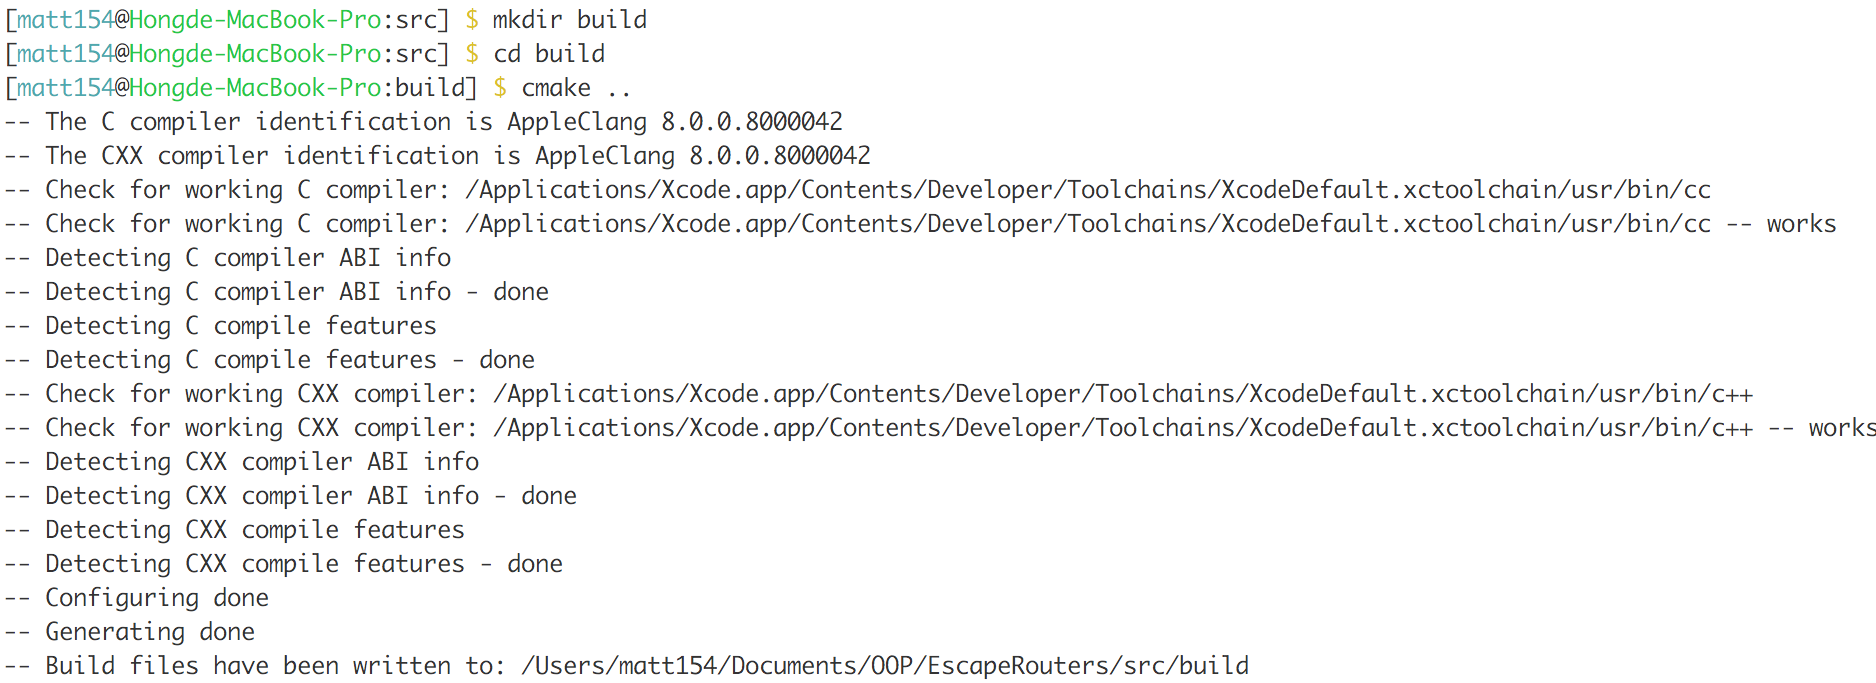
\includegraphics[width = 0.8\textwidth]{test0.png}
        \caption{Building (CMake)}
    \end{figure}
    \begin{figure}[H]
        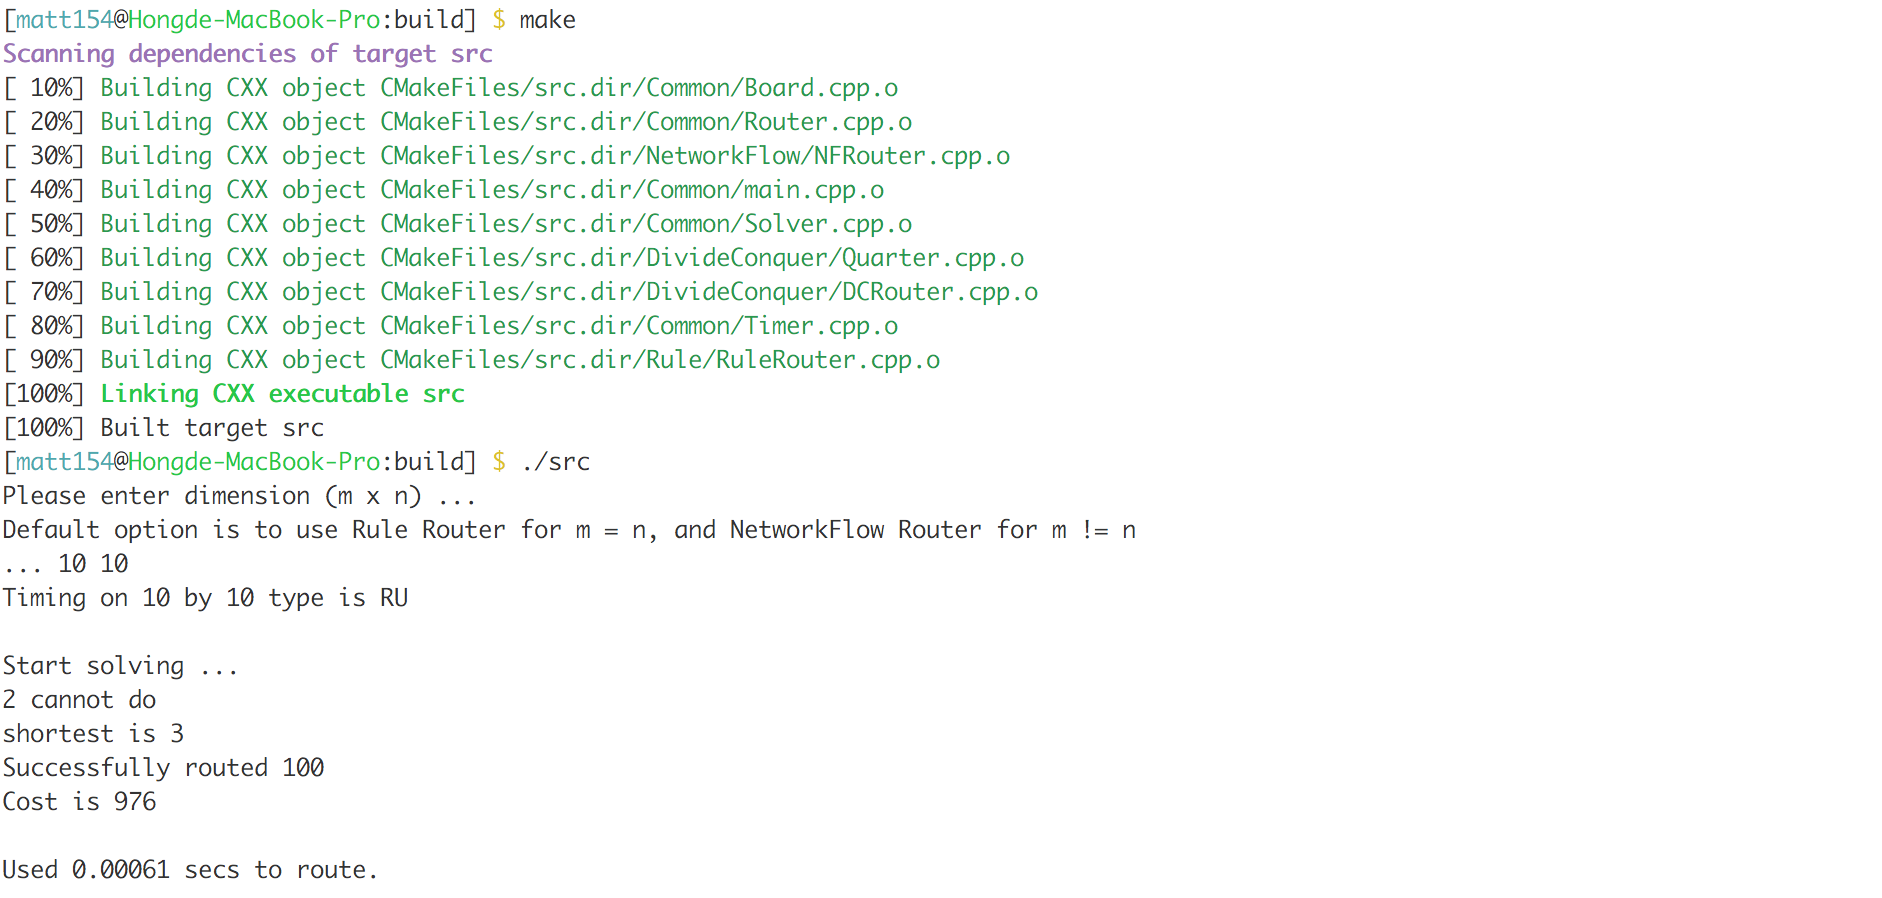
\includegraphics[width = 0.8\textwidth]{test1.png}
        \caption{Making \& testing}
    \end{figure}
    \subsubsection{Visualizer}
    \label{VIS}
    The visualizer can display the routed board with different scales.
    \begin{figure}[H]
        \centering
        \begin{subfigure}{0.25\textwidth}
            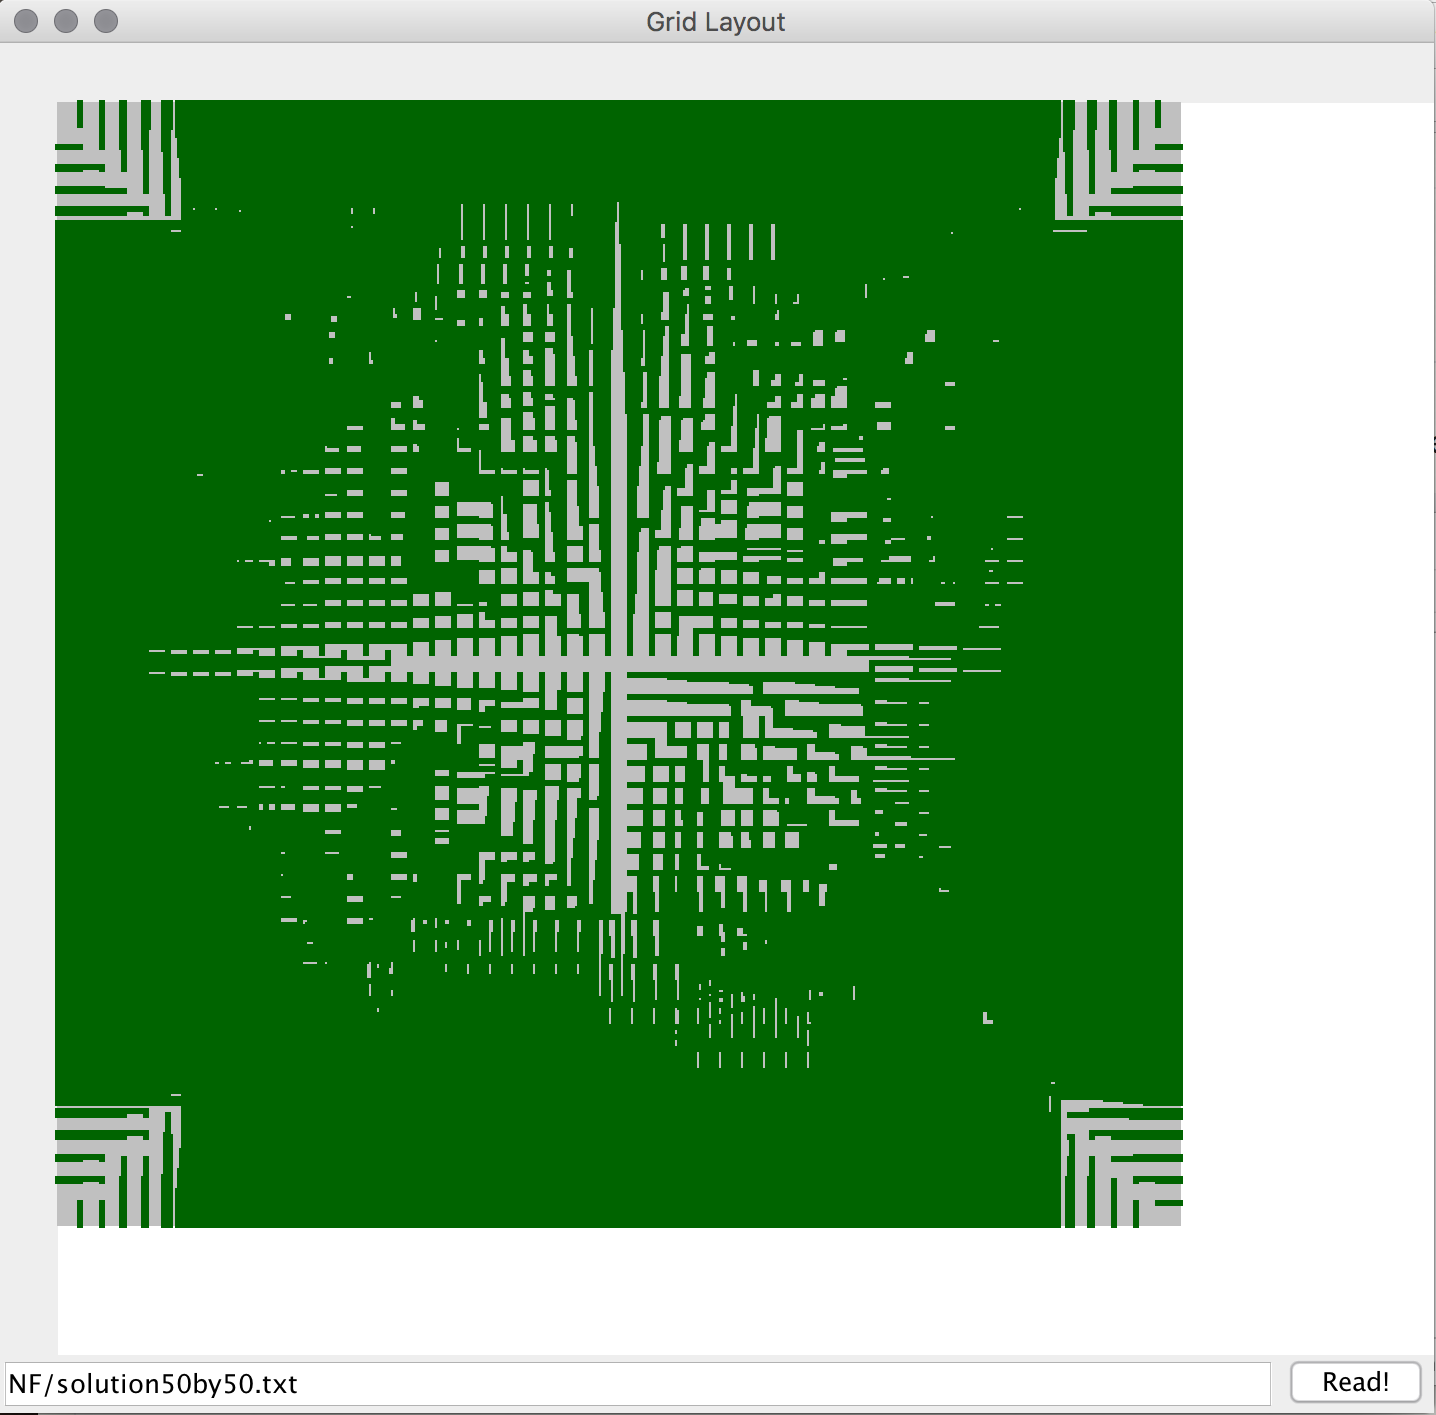
\includegraphics[width = \textwidth]{vis1.png}
            \caption{1x}
        \end{subfigure}
        \begin{subfigure}{0.25\textwidth}
            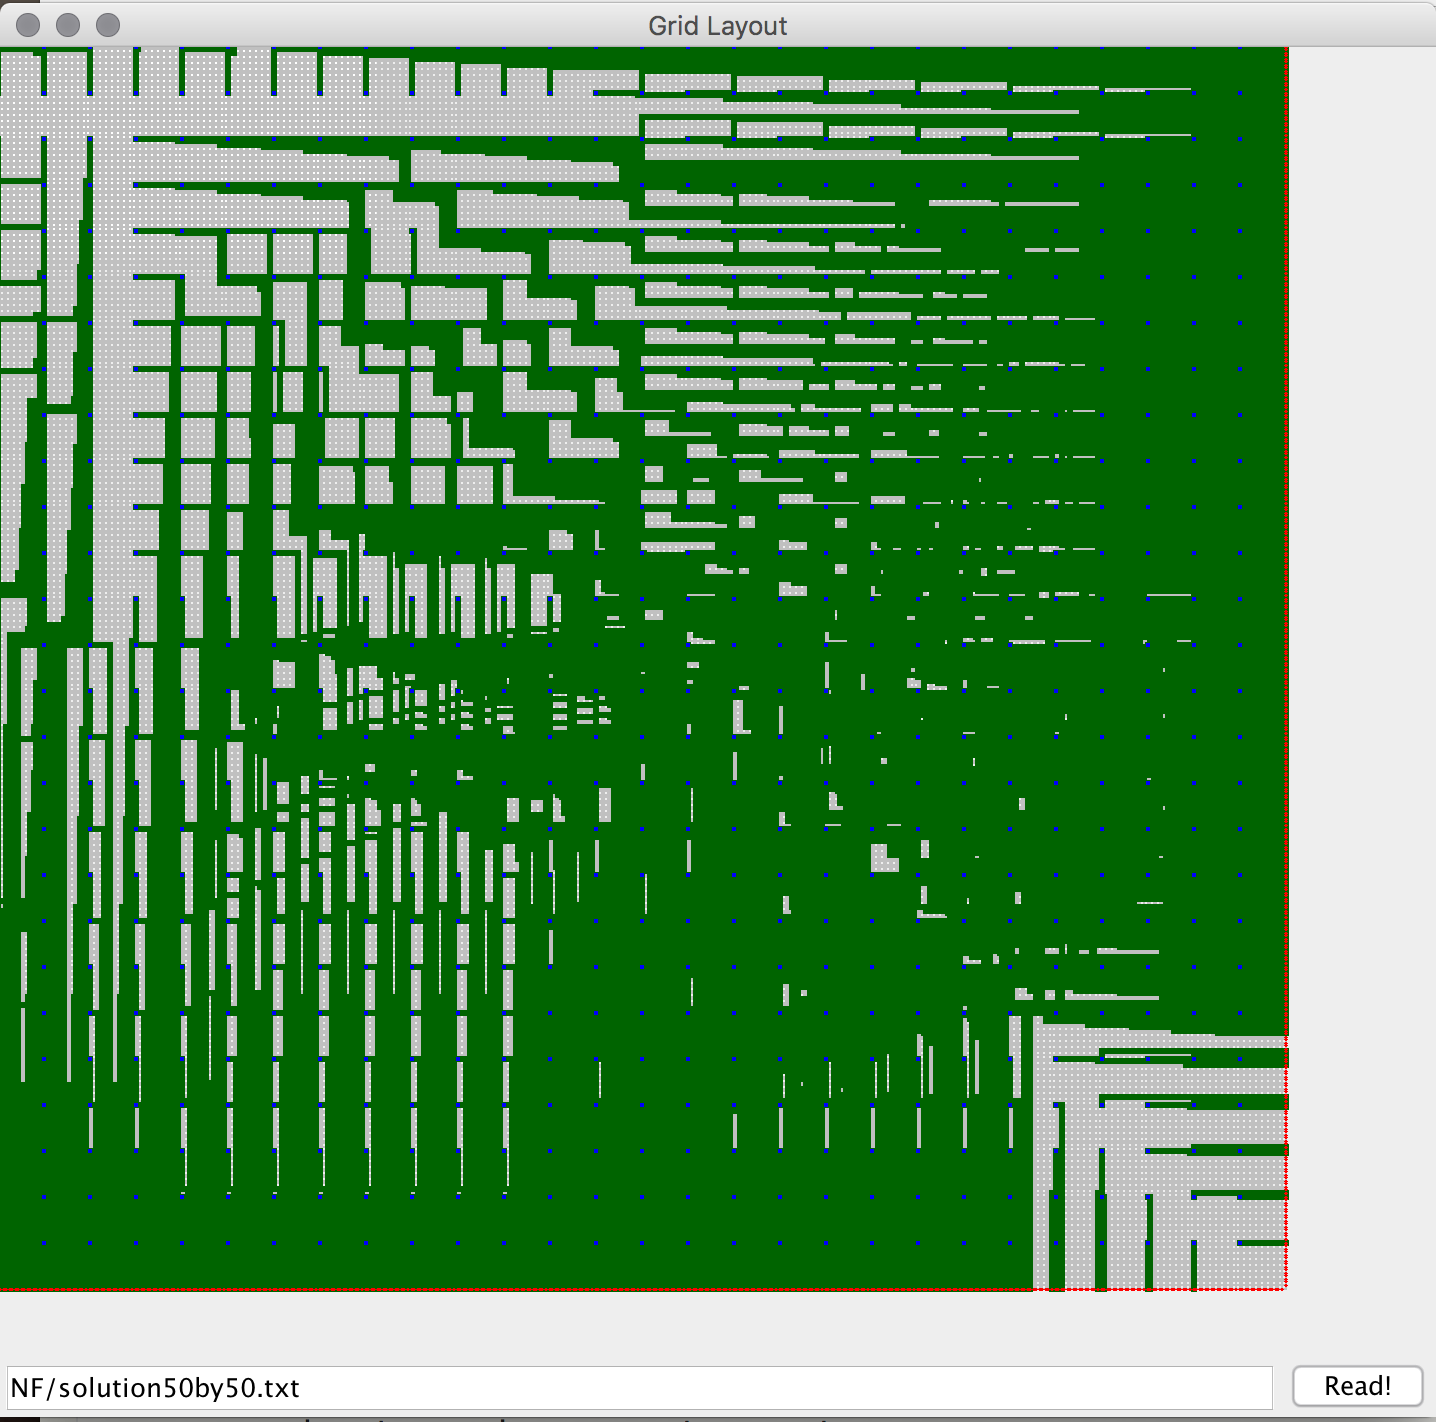
\includegraphics[width = \textwidth]{vis2.png}
            \caption{2x}
        \end{subfigure}
        \begin{subfigure}{0.25\textwidth}
            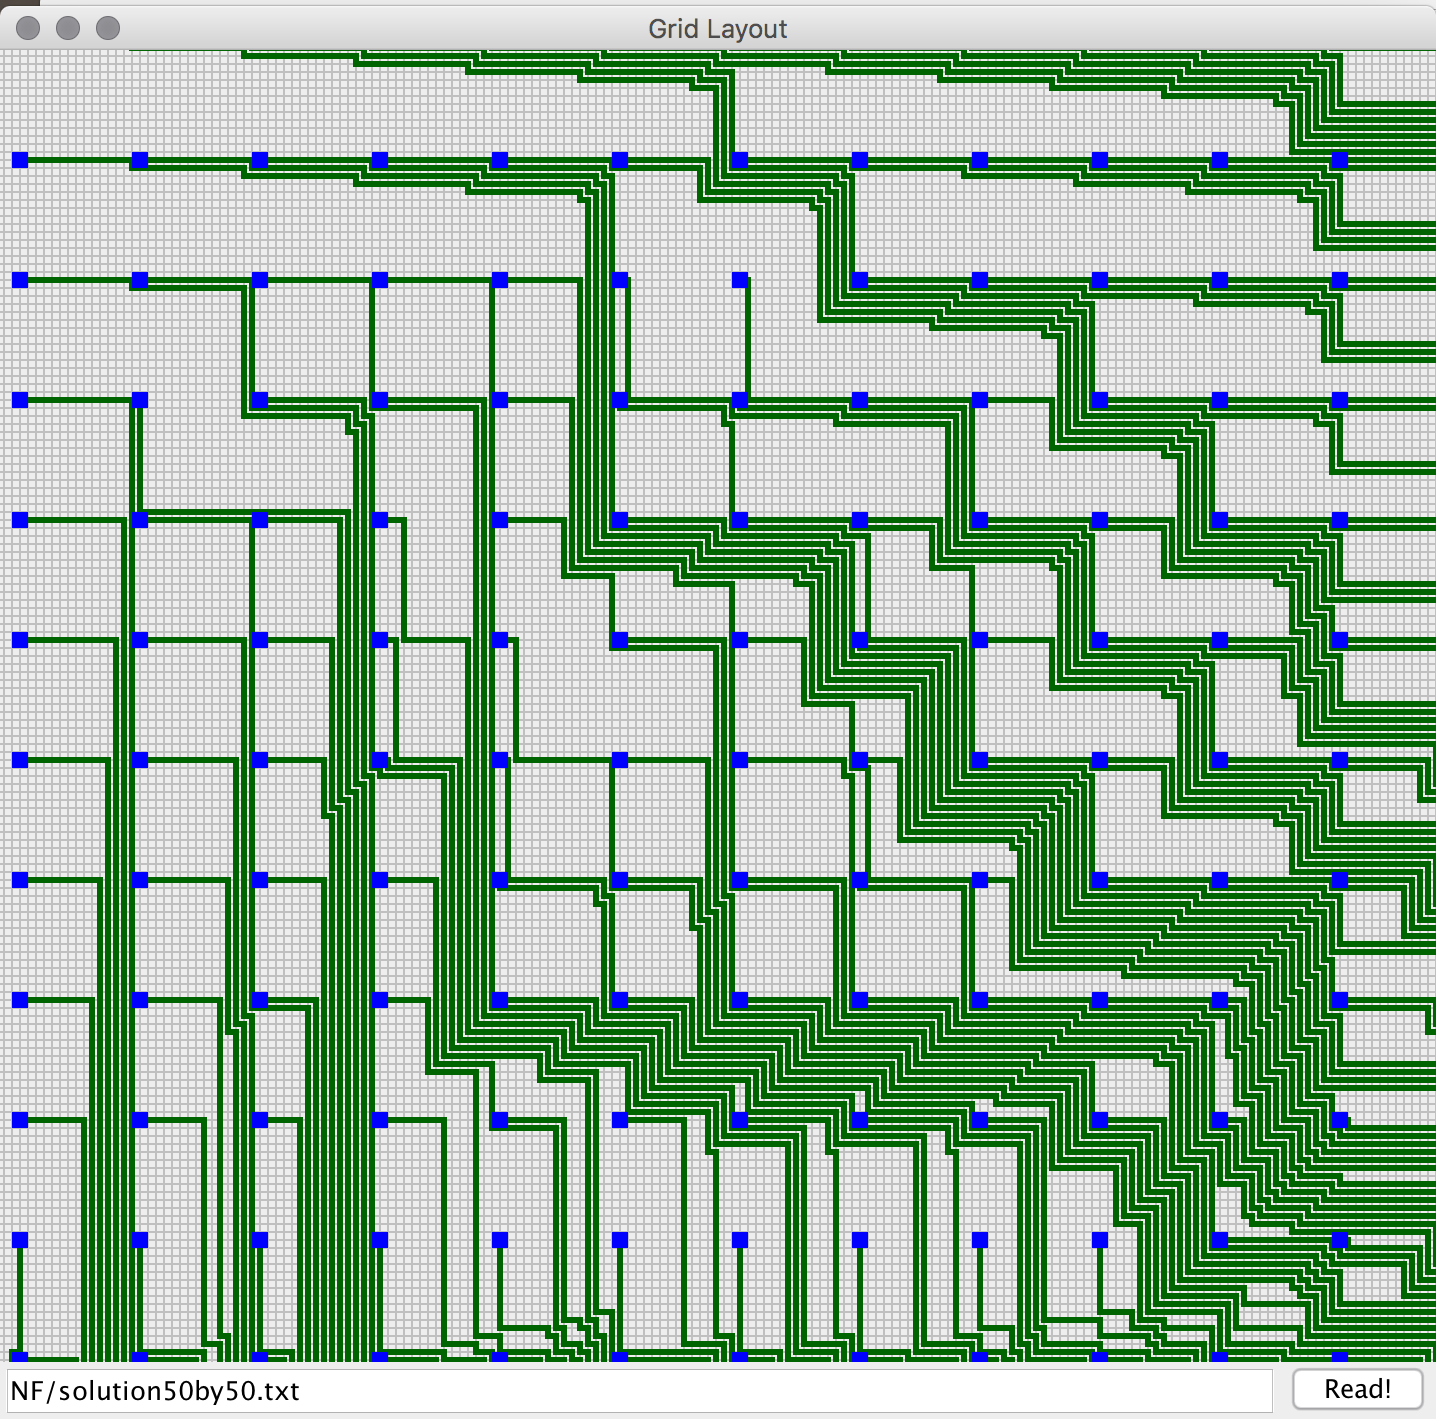
\includegraphics[width = \textwidth]{vis3.png}
            \caption{4x}
        \end{subfigure}
        \caption{Visualizer, with NF router results}
    \end{figure}
    The usage is simple, to zoom in near a specific point, left click. To return to original scale, right click. Notice that the image is zoomed in with the position clicked at the upper left corner.
    \newpage
    \section{Overview}
    In this project, an escape routing problem is solved using three approaches, each with different performance and limitation. The escape routing problem is given as follows.

    Given equally spaced internal node array
    \begin{enumerate}[label = \alph*]
        \item find the smallest number $k$ of ``gap'' lines between the nodes, such that the nodes can connect to terminal nodes with non-crossing paths.
        \item Furthermore, find the shortest routing paths if possible.
    \end{enumerate}
    \begin{figure}[H]
        \centering
        \begin{subfigure}{0.3\textwidth}
            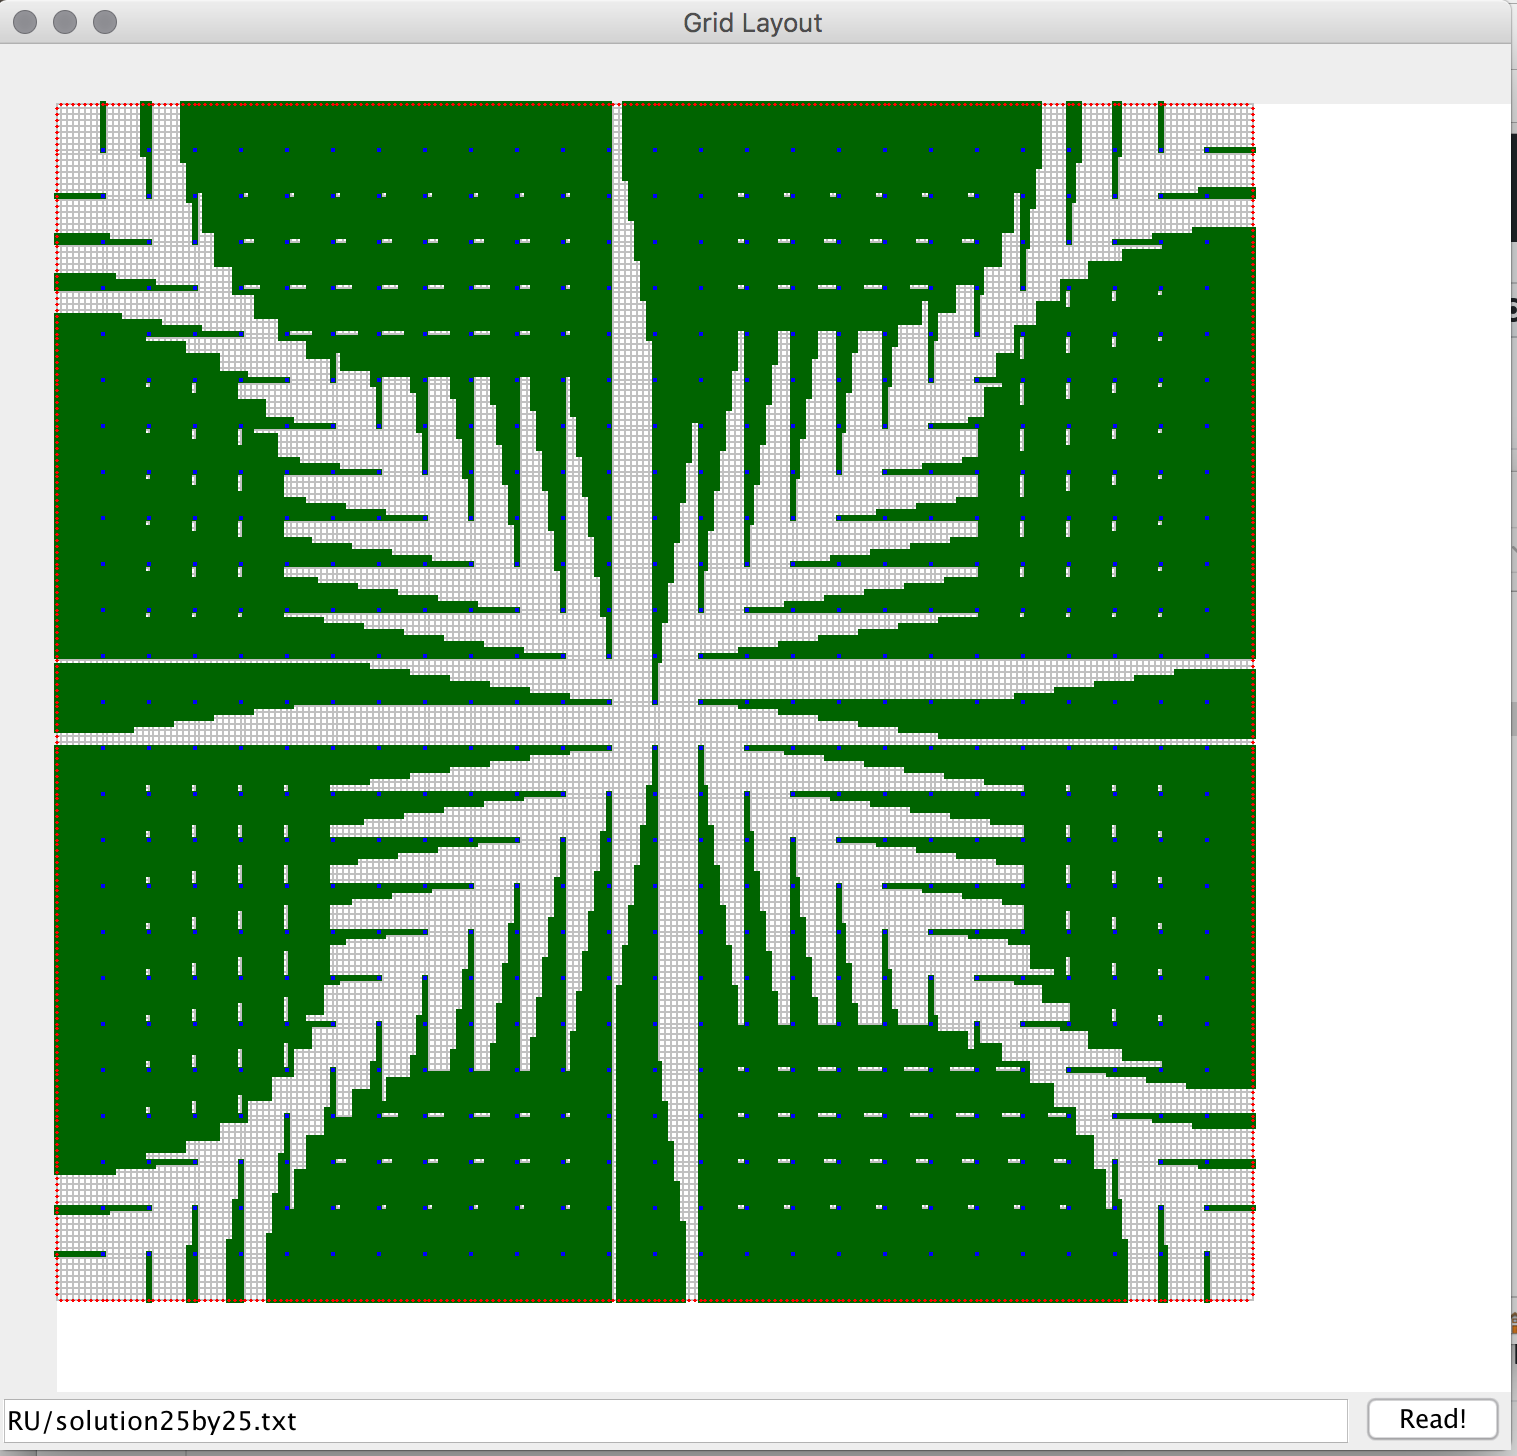
\includegraphics[width = \textwidth]{ove1.png}
            \caption{RuleRouter (20 x 20)}
        \end{subfigure}
        \begin{subfigure}{0.3\textwidth}
            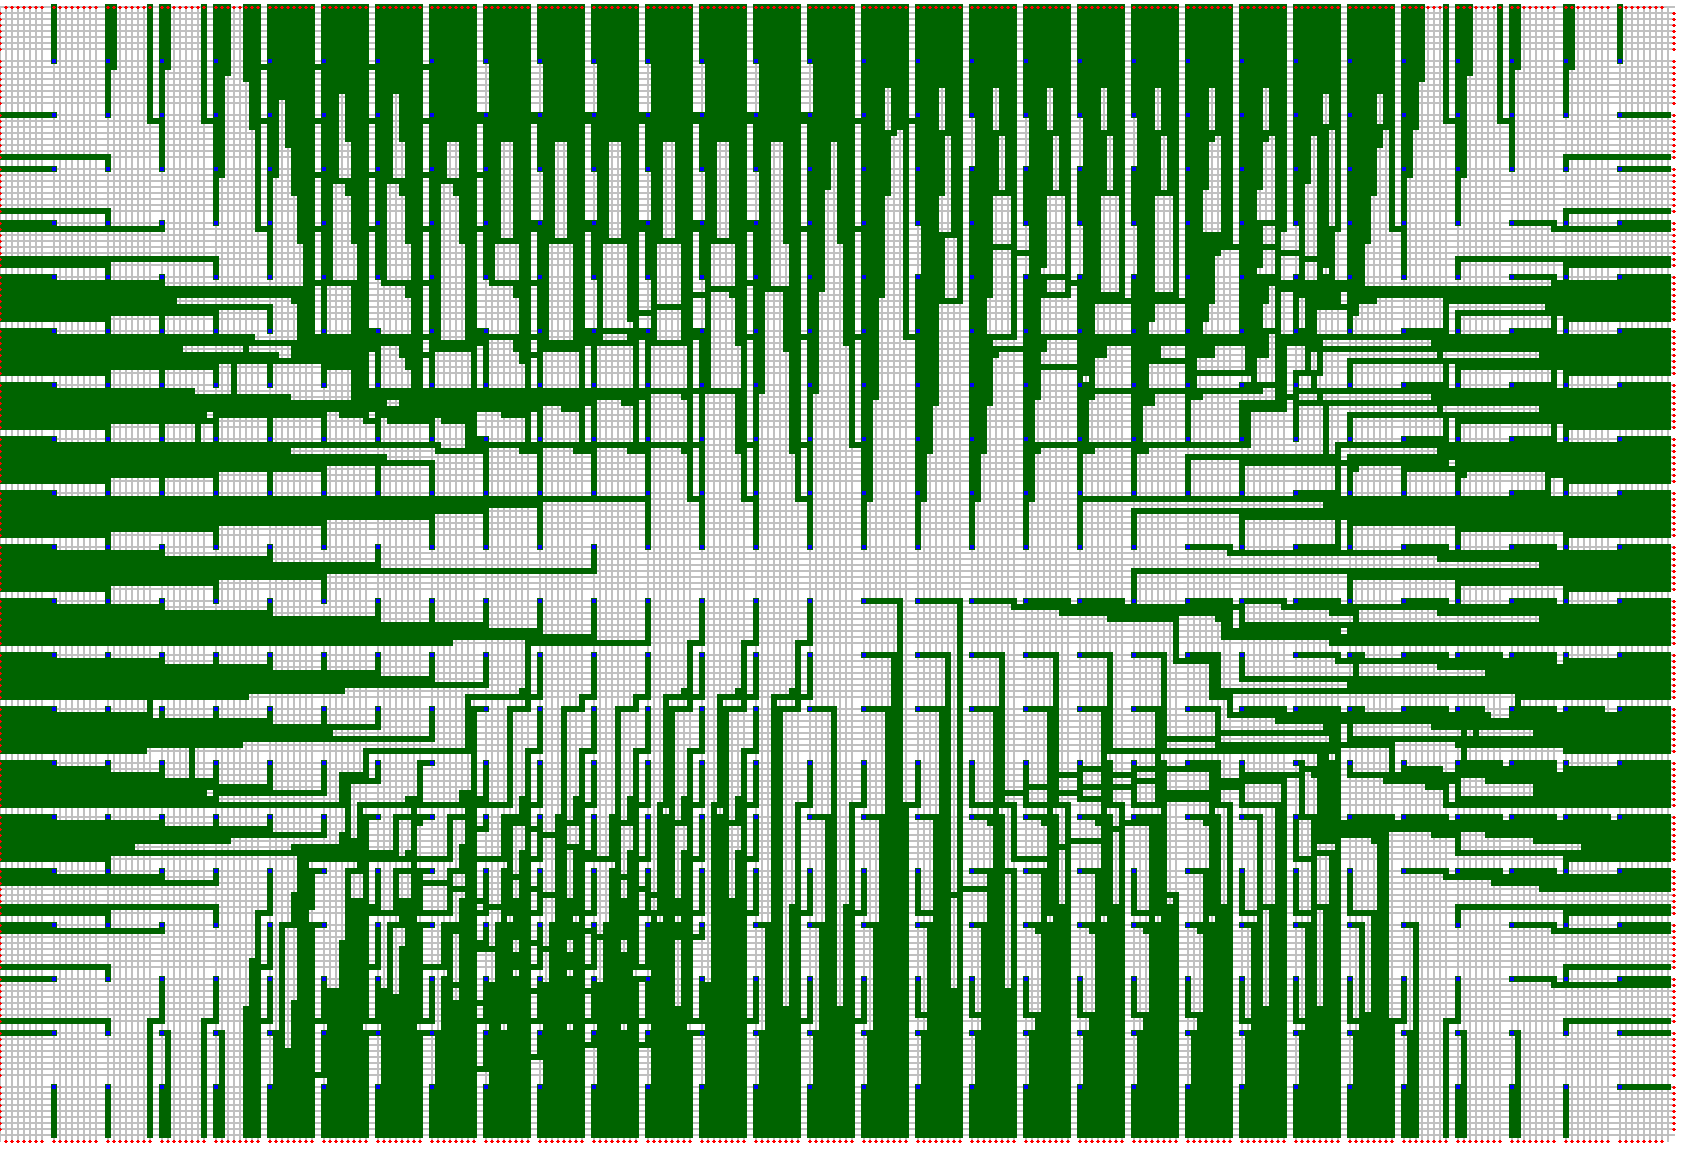
\includegraphics[width = \textwidth]{ove2.png}
            \caption{NFRouter (20 x 30)}
        \end{subfigure}
        \begin{subfigure}{0.3\textwidth}
            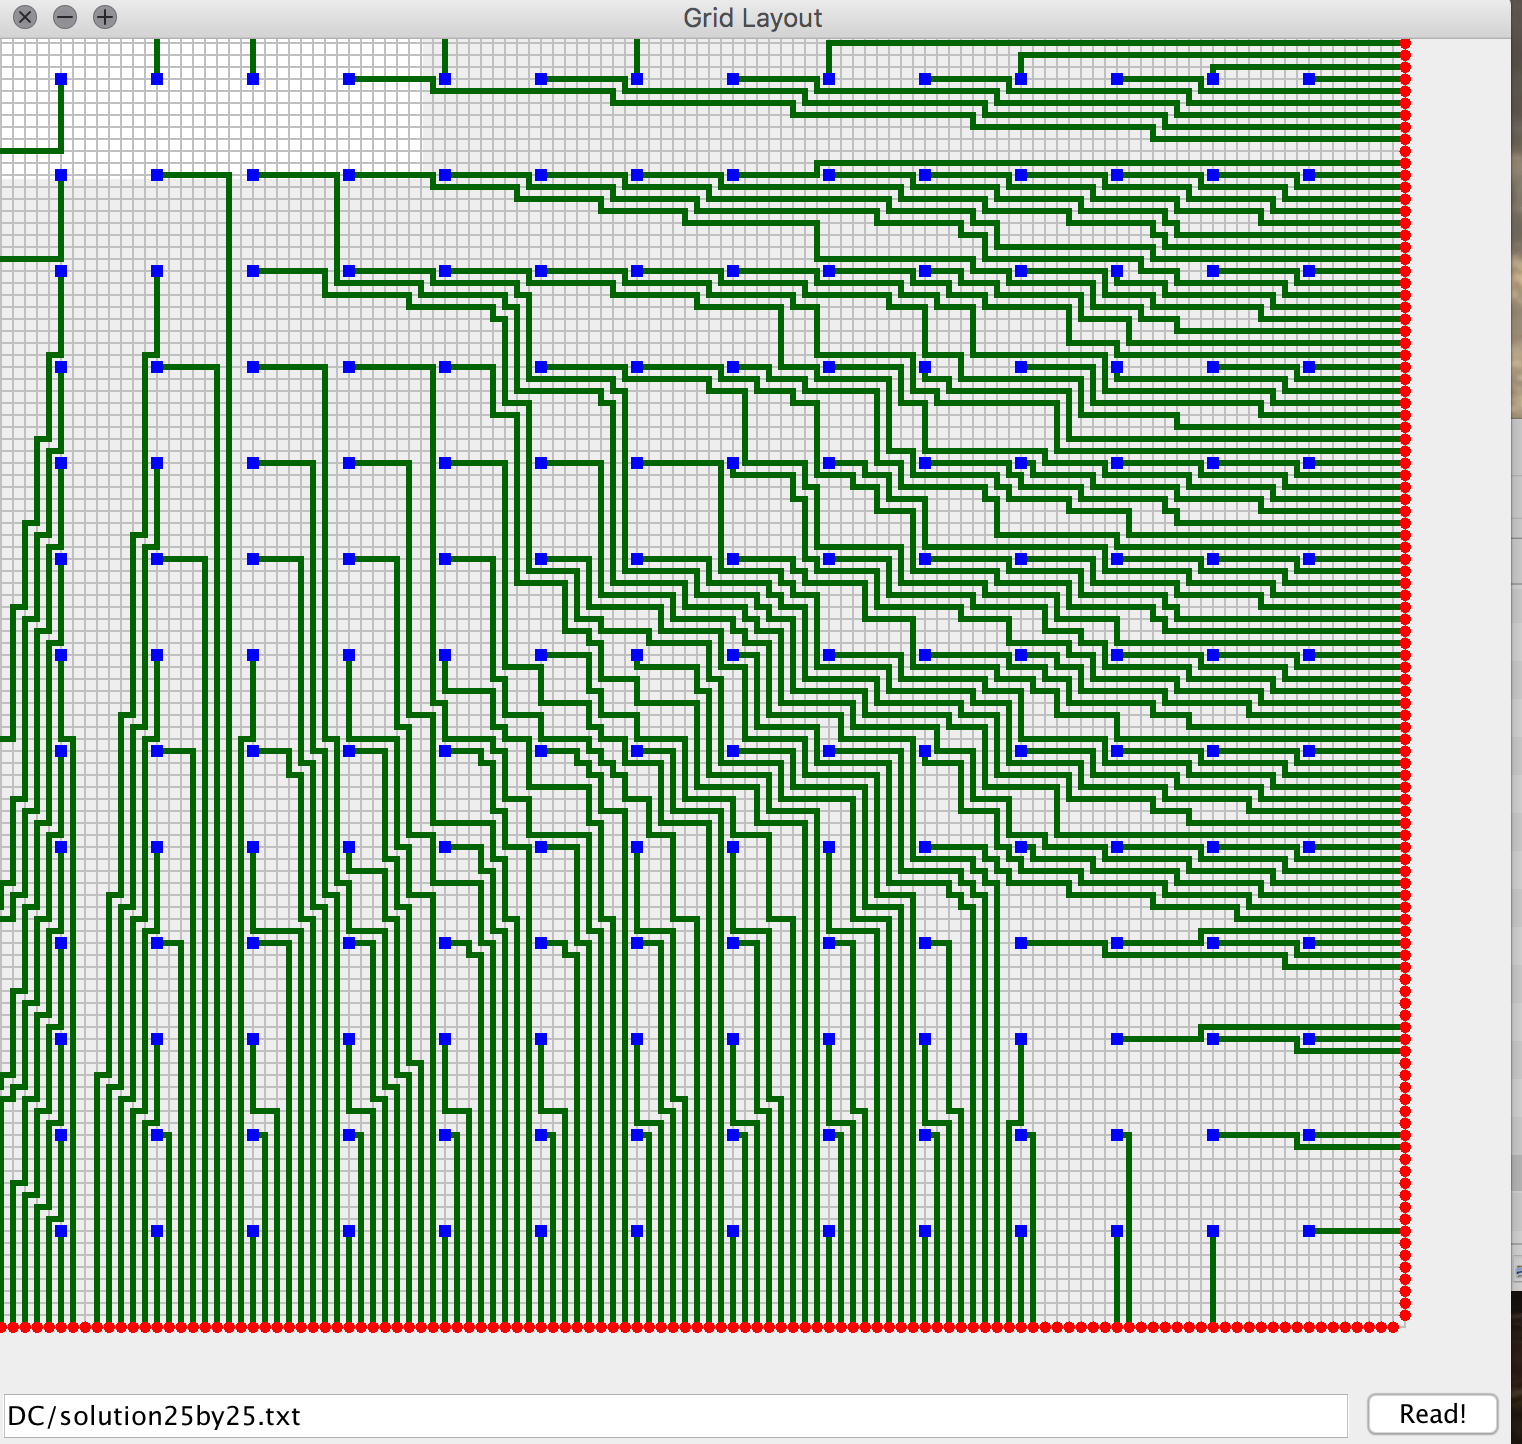
\includegraphics[width = \textwidth]{ove3.png}
            \caption{Partial solution}
        \end{subfigure}
        \caption{Different routing solutions}
    \end{figure}
    In this project, the number of nodes is assumed to be about 400 ($20 \times 20$) to $\sim$5000 ($70 \times 70$). However, other number of nodes (e.g. $100 \times 100$) can also be handled by the solvers, see the test data
    for details.
    \section{Data Representation}
    \subsection{Board format}
    \label{DAT:BOARD}
    Each board is encapsulated by a Board object, which keeps track of the size of the problem ($N, M, K$, the height, width and gap respectively) and the real dimesion of the board ($DM, DN$). In each grid of the board, a
    number from $\{0, 1, 2, 3, 4\}$ is kept, which tells the direction of the edge from that grid. An example is illustrated below.
    \begin{figure}[H]
        \centering
        \begin{subfigure}{0.4\textwidth}
            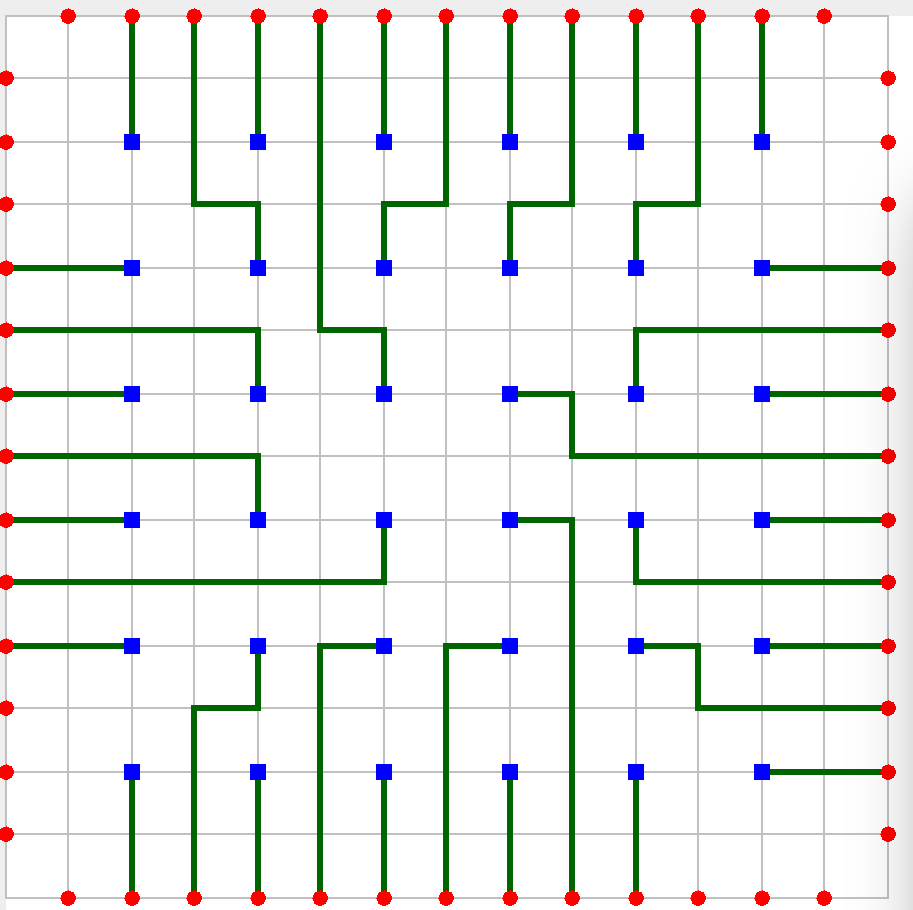
\includegraphics[width = \textwidth]{dat1.png}
            \caption{Board}
        \end{subfigure}
        \begin{subfigure}{0.4\textwidth}
            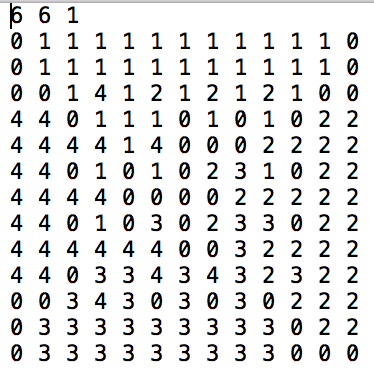
\includegraphics[width = \textwidth]{dat2.png}
            \caption{Digital Board}
        \end{subfigure}
        \caption{Board representation}
    \end{figure}
    \subsection{Internal Object Design}
    The whole project is divided into four modules, the most important of which is the Common module. More implementation details and algorithms are explained in Section \ref{RA}.
    \subsubsection{Common}
    In the common module, several basic objects are stored.
    \paragraph{Board}
    Board class is already discussed in Section \ref{DAT:BOARD}
    \paragraph{Router}
    Router class is a template class for the routing process, it has two virtual methods. Function OK() returns whether the board is routable, and function route() returns a pointer to a solution board, or NULL if it does not exist.
    \paragraph{Solver}
    The solver, along with router class, implements a strategy pattern. It uses incremental search for $K$ (starting from $\floor{\frac{n}{4}} - 1$) instead of binary search, because by experiment $k$ is commonly 2 or 3 apart.
    \paragraph{Timer}
    The timer uses the solver class and can be seen as a proxy. Its purpose is to keep log of the results and do output.
    \paragraph{Java/Drawer}
    The drawer is written in Java Swing and do visualization, explained in Section \ref{VIS}.
    \subsubsection{NetworkFlow}
    In the NetworkFlow module is stored the implementation of NFRouter. It utilizes network flow formulation.
    \subsubsection{DivideConquer}
    In the DivideConquer module is stored the DCRouter, which uses divide and conquer technique to speed up solution. Another class Quarter, which is a modification of NFRouter by inheritance, is stored in the module and used by DCRouter.
    \subsubsection{Rule}
    The RuleRouter, which is the fastest router, is stored in this module.
    \section{Routing approaches}
    The routing approahes are explained briefly in this section. For more implementation details please consult $/src$. The performances and correctness are dicussed in Section \ref{STAT}.

    It is easy to prove that minimum gap is at least $\floor{\frac{n}{4}} - 2$ for square boards.

    \begin{proof}
        There are $n^2$ internal nodes, and $kn + n + k$ terminals on each edge. Therefore
        \begin{align*}
            4kn + 4n + 4k &\ge n^2\\
            k &\ge \frac{n^2 - 4n}{4n + 4}\\
            k &\ge \frac{n^2 + n}{4n + 4} - \frac{5n}{4n + 4} \ge \frac{n}{4} - 2
        \end{align*}
    \end{proof}

    By experiment this gap is not too far away from $\floor{\frac{n}{4}} - 2$, so using incremental search can be more efficient than binary search.
    \label{RA}
    \subsection{Network Flow}
    The formulation to network flow is straightforward. The first approach is to treat every intersection point of the board as a node on the network flow graph, and add a ``super source'' connected to every internal nodes, a ``super sink'' connected to every
    node on the boundary. Every edge between the nodes have capacity one, and our goal is to make the flow $M \times N$.

    However, the above formulation only forbids the same edge to be used twice, which does not actually forbid ``crossing paths'' on the board. Also, the formulation cannot deal with the total length. So another formulation using minimum cost flow is invented.

    The correct approach is to assign the capacity 1 to both the nodes and the edges, and a cost of 1 to the nodes. Nodes with capacities and costs are implemented in a classical way -- by splitting a node into an ``in'' node and an ``out'' node, and connecting them by
    an edge with capacity 1 and cost 1. Note that the length of the escaping path is correctly recorded by the number of nodes it passed through.

    Having a correct formulation, we implemented the augmenting shortest path algorithm, which uses label-correcting algorithm, as dicussed on this site \cite{FLOW}.

    Several outputs are the following. Note that this router can not only handles squares, but also rectangles.
    \begin{figure}[H]
        \centering
        \begin{subfigure}{0.3\textwidth}
            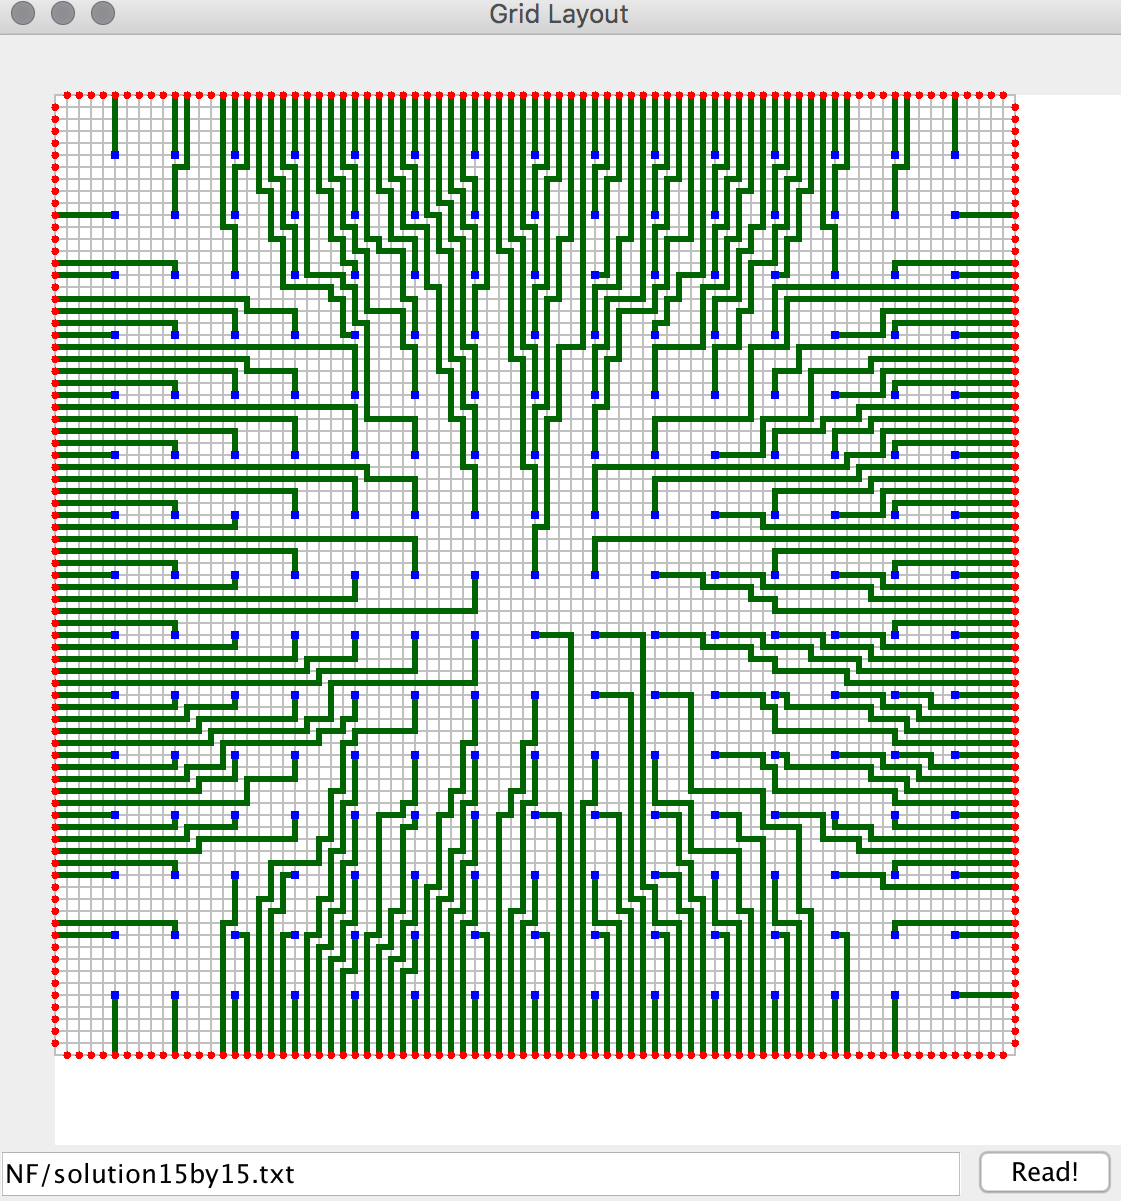
\includegraphics[width = \textwidth]{NF1.png}
            \caption{15 x 15}
        \end{subfigure}
        \begin{subfigure}{0.3\textwidth}
            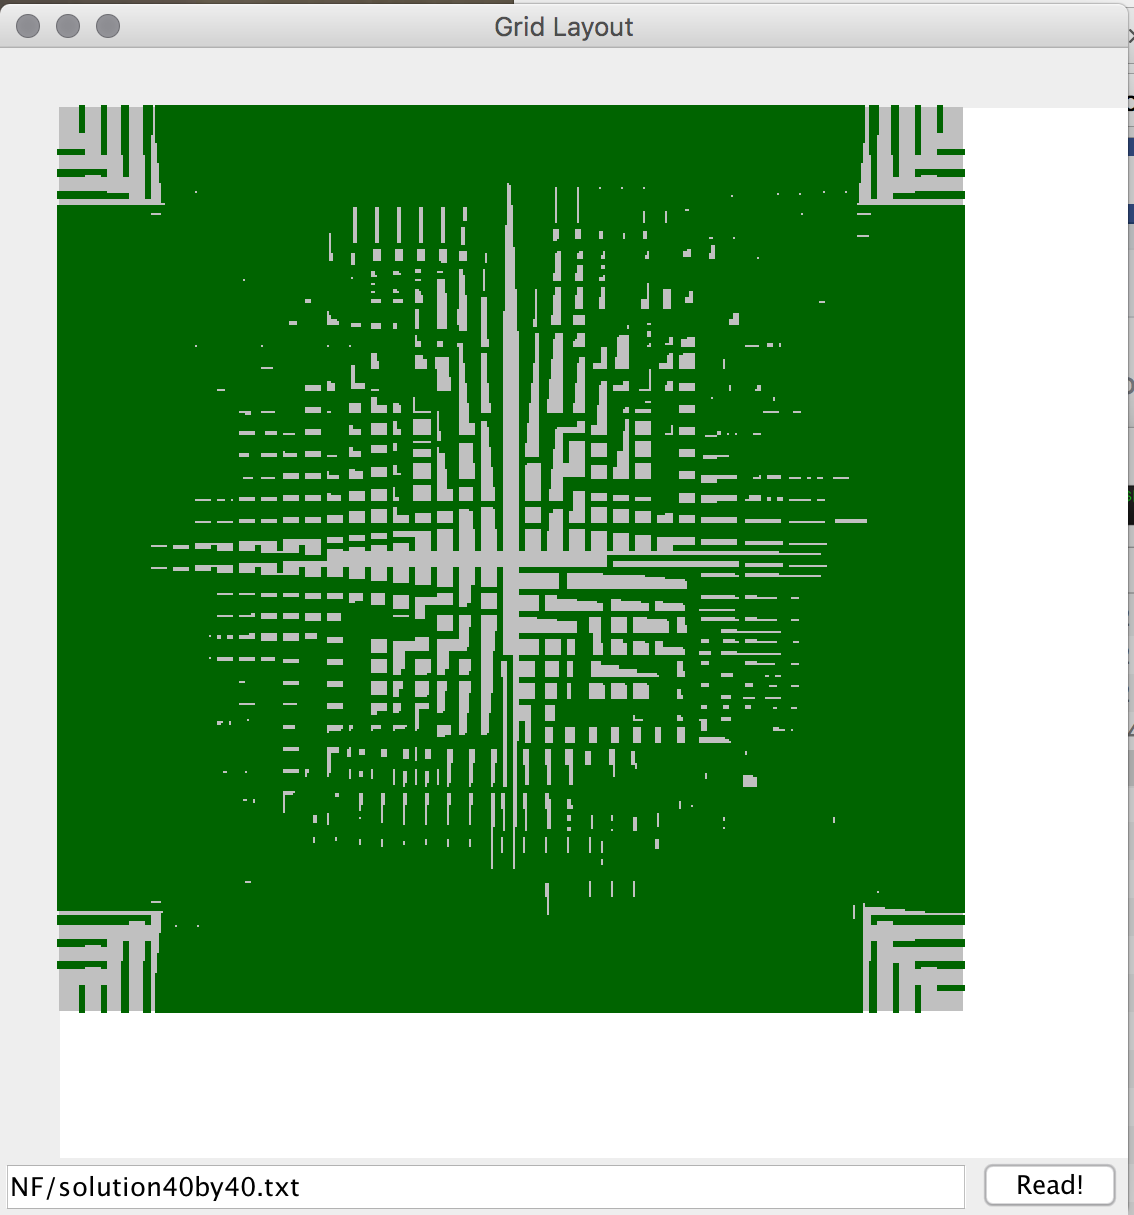
\includegraphics[width = \textwidth]{NF2.png}
            \caption{40 x 40}
        \end{subfigure}
        \begin{subfigure}{0.3\textwidth}
            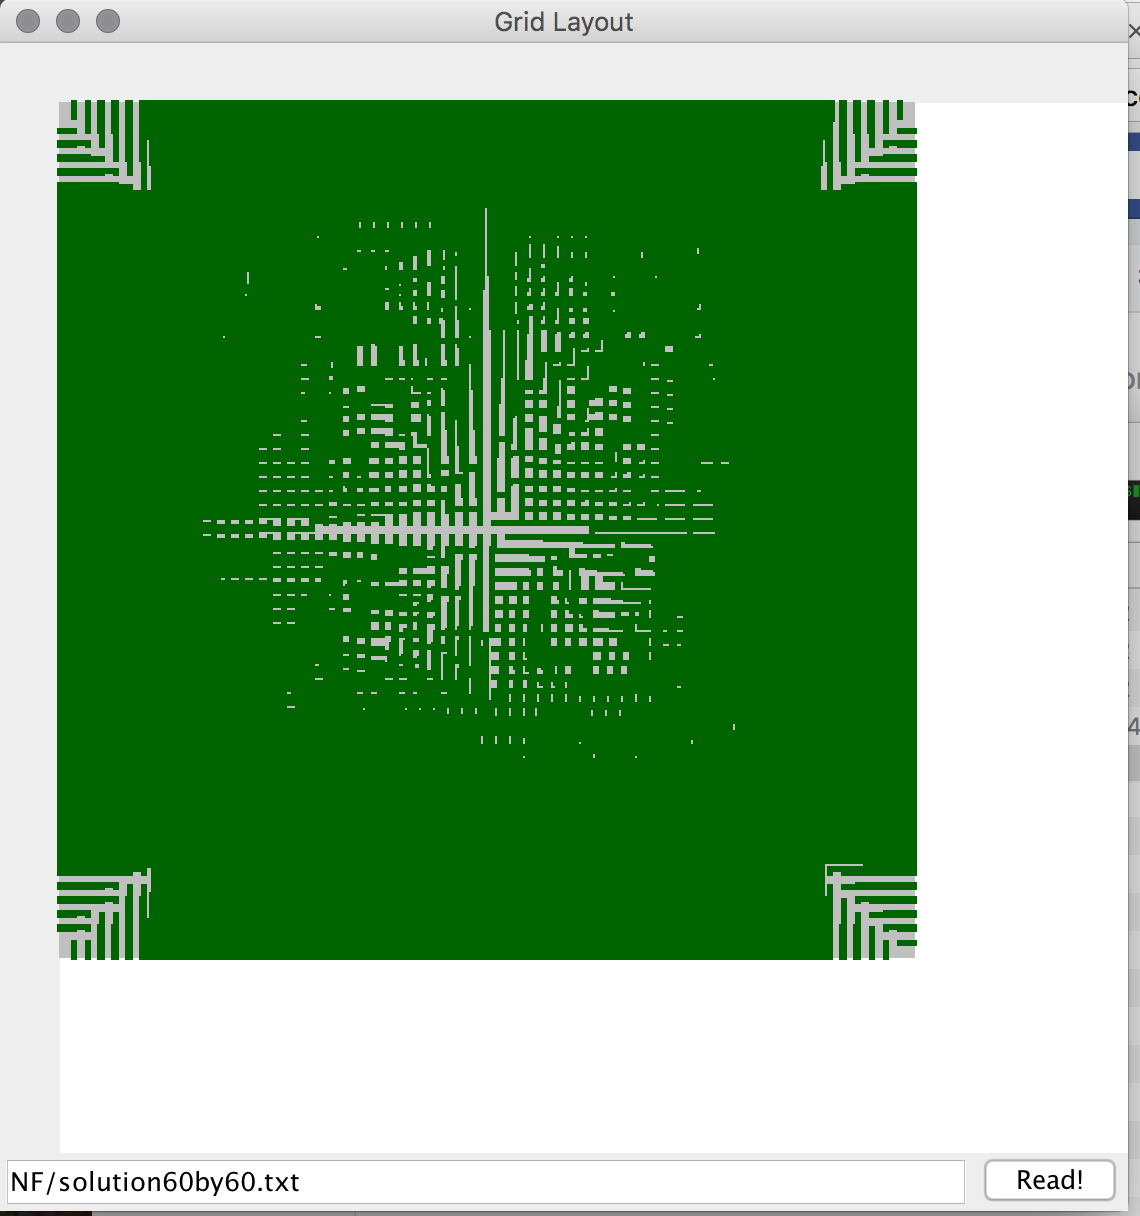
\includegraphics[width = \textwidth]{NF3.png}
            \caption{60 x 60}
        \end{subfigure}
        \caption{NFRouter with different sizes}
    \end{figure}
    \subsection{Divide and Conquer}
    \label{DC}
    After studying the solution from NFRouters, we found that optimal solutions for squares have some special properties. One such properties is that the four corners are sparse and the other regions are extremely dense. However, this property
    might not be so useful for speeding up the solution.

    Squares are special in that the are more regular and symmetric compared to rectangles, and we found that the solutions also have some sort of symmetry for the four corners. It seems that we can divide the whole board into four regions, solve for
    one quarter, and rotate the solution to get the whole results. This leads us to the DCRouter.

    To implement such an approach and do better code reuse, we have class Quarter inherit from NFRouter. We can use the same routing function, and only need to modify the add\_edge() and fulfill() methods, which are designed for modification, to make the underlying graph different.

    Detail implementations includes even-odd case analysis and are not covered in this documentation. It is worth noting that after Quarter behaves correctly, what is left is to do rotation.

    Theoretically this approach can speed up the efficiency of network flow by a constant factor ($\sim 4^2 = 16$). In reality DCRouter is about 20 times faster.

    Another thing to be noted is that, when $n$ is odd, $DC$ router returns suboptimal length ($k$ is optimal) because the center point cannot be easily divided into any quarter. For even size, the router behaves optimal as verified by NFRouter.
    \begin{figure}[H]
        \centering
        \begin{subfigure}{0.3\textwidth}
            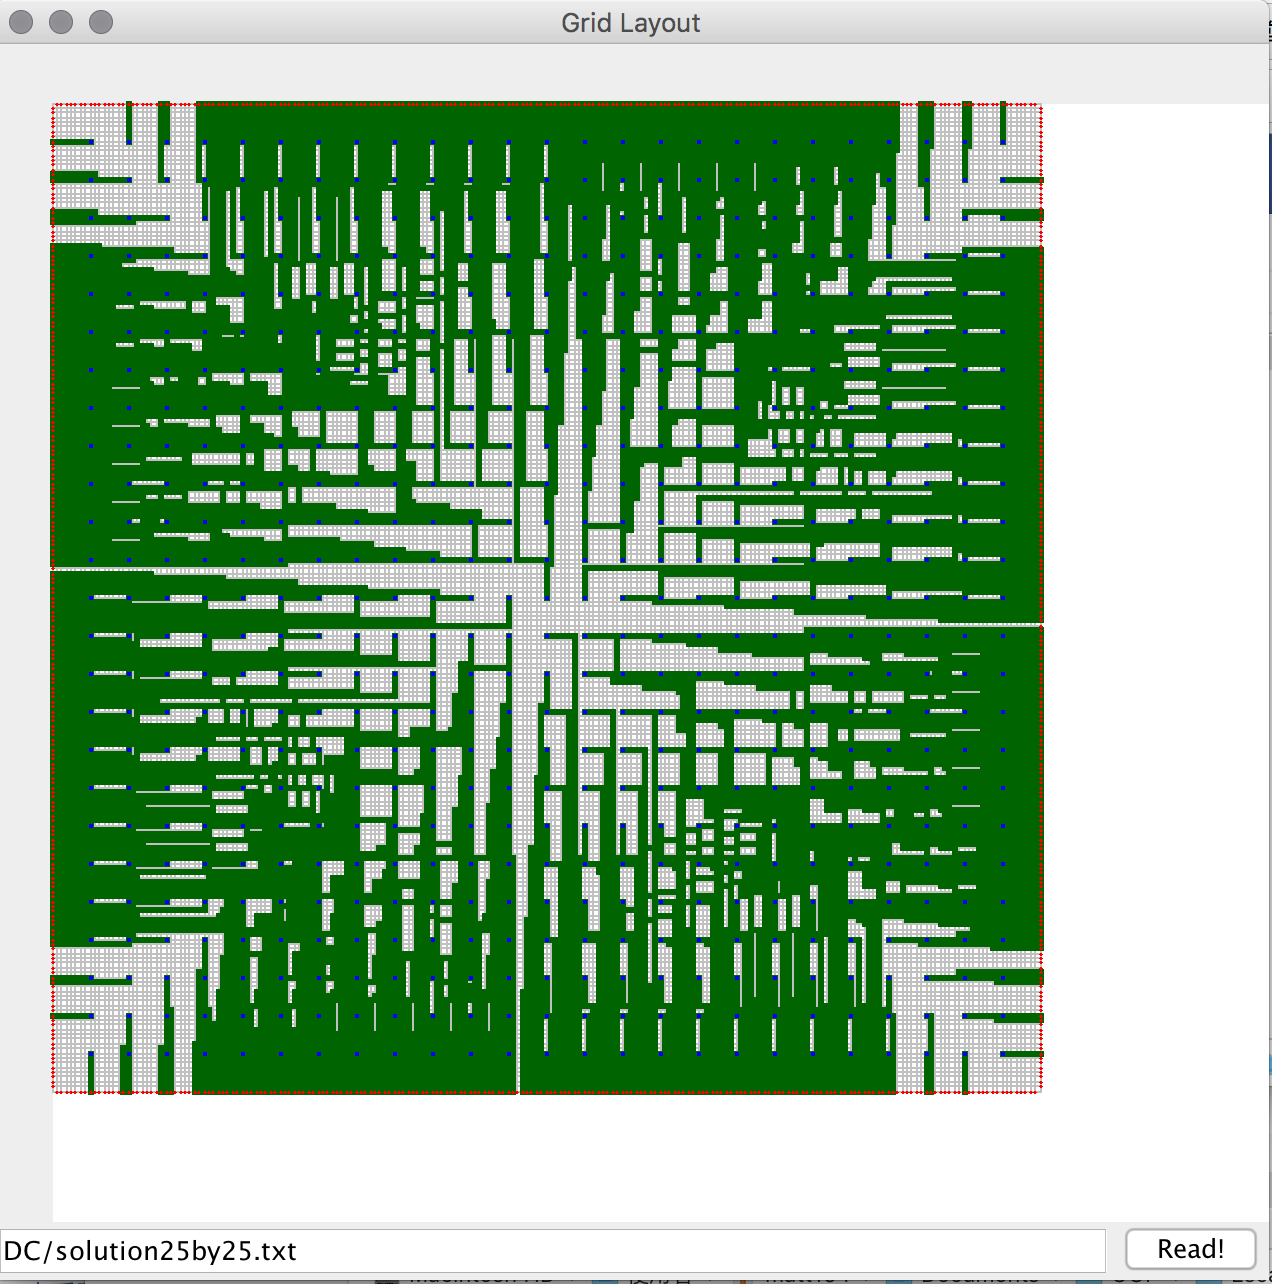
\includegraphics[width = \textwidth]{DC1.png}
            \caption{25 x 25}
        \end{subfigure}
        \begin{subfigure}{0.3\textwidth}
            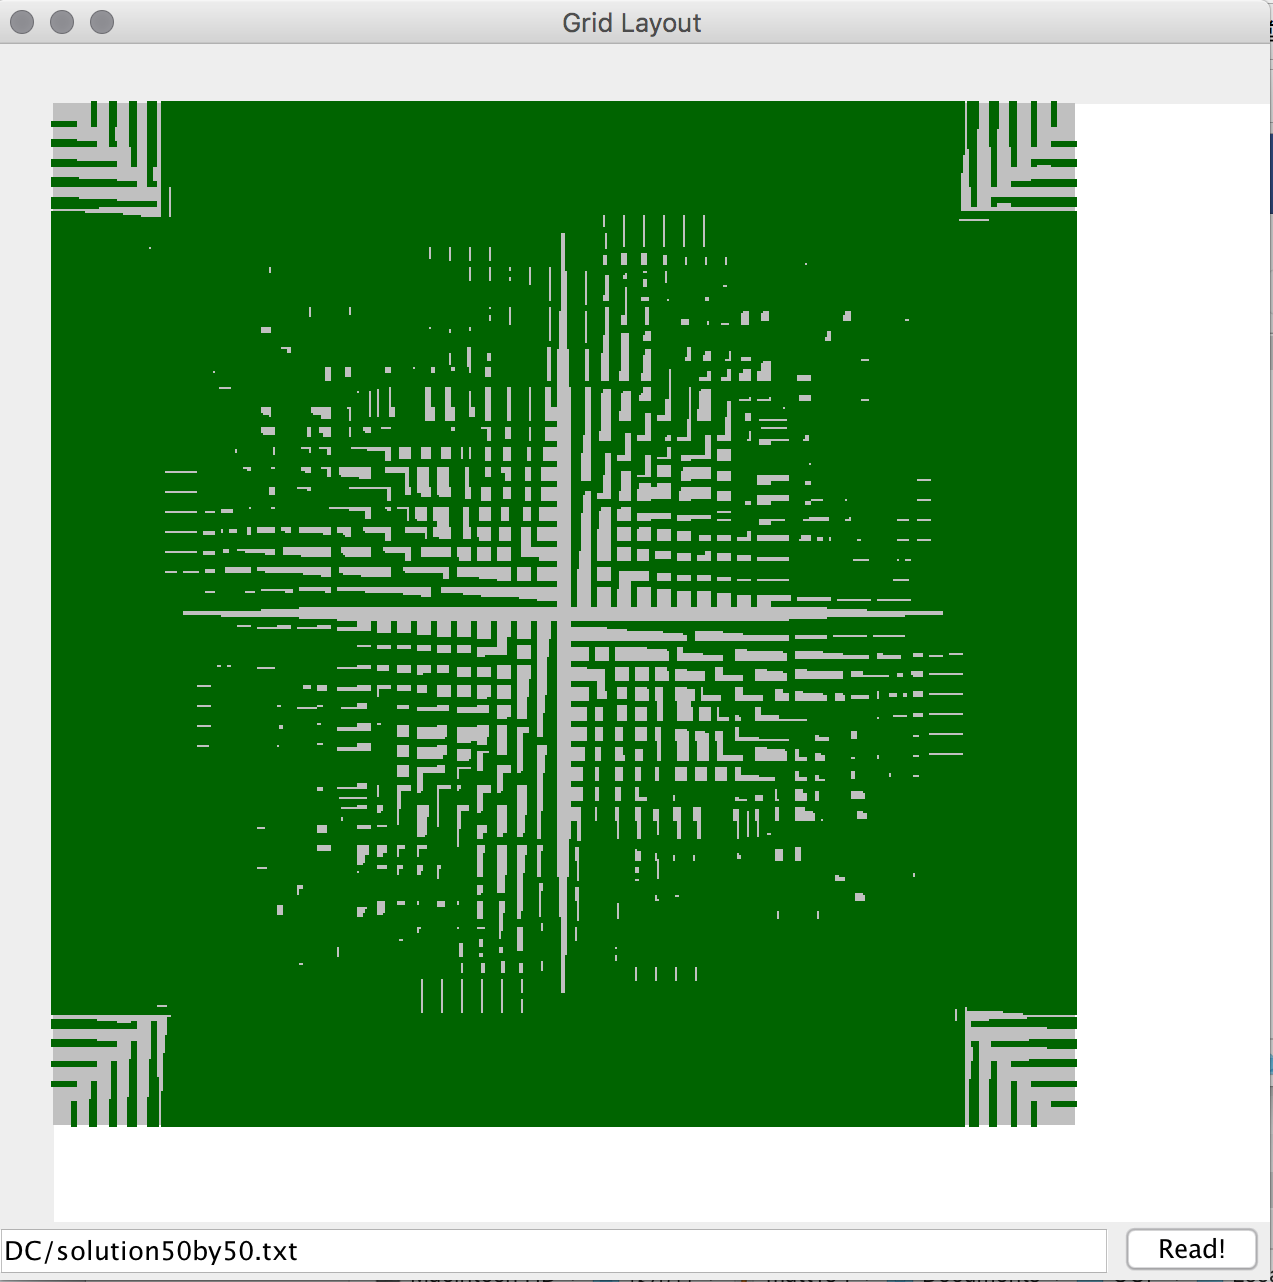
\includegraphics[width = \textwidth]{DC2.png}
            \caption{50 x 50}
        \end{subfigure}
        \begin{subfigure}{0.3\textwidth}
            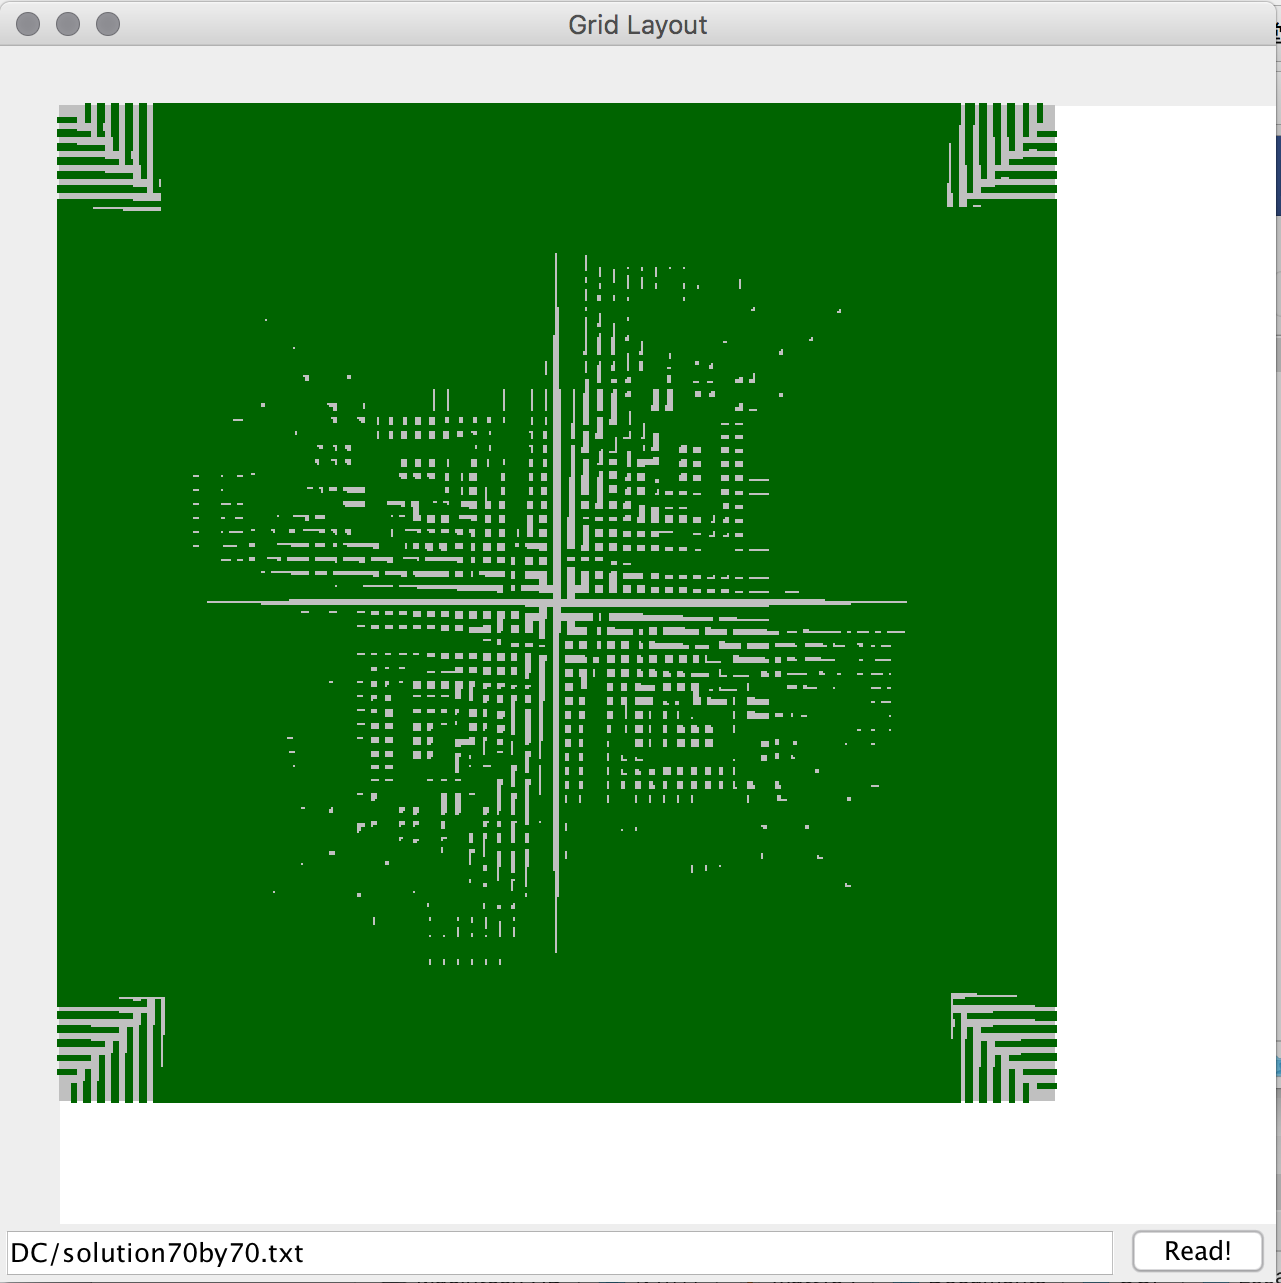
\includegraphics[width = \textwidth]{DC3.png}
            \caption{70 x 70}
        \end{subfigure}
        \caption{DCRouter with different sizes}
    \end{figure}
    \subsection{Rule Based Method}
    \subsubsection{Observations}
    The previous two methods have a worst case complexity of $O(f VE) = O(n \times n^8) = O(n^9)$, but normally runs in $\sim O(n^5)$. However, these complexities are not affordable as $n$ grows large. So we proposed a rule-based routing methods, which utilizes the symmetry of squares.

    We have mentioned that, it seems that the paths can be safely divided into four quarters. This suggestion is verified by DCRouter results in\ref{DC}. Nevertheless, points at the boundary of the quarters may not be able to be properly distributed. This leads us to think of another way
    of dividing the board -- by the diagonal. Let's take a closer look at the NF solution.

    \begin{figure}[H]
        \centering
        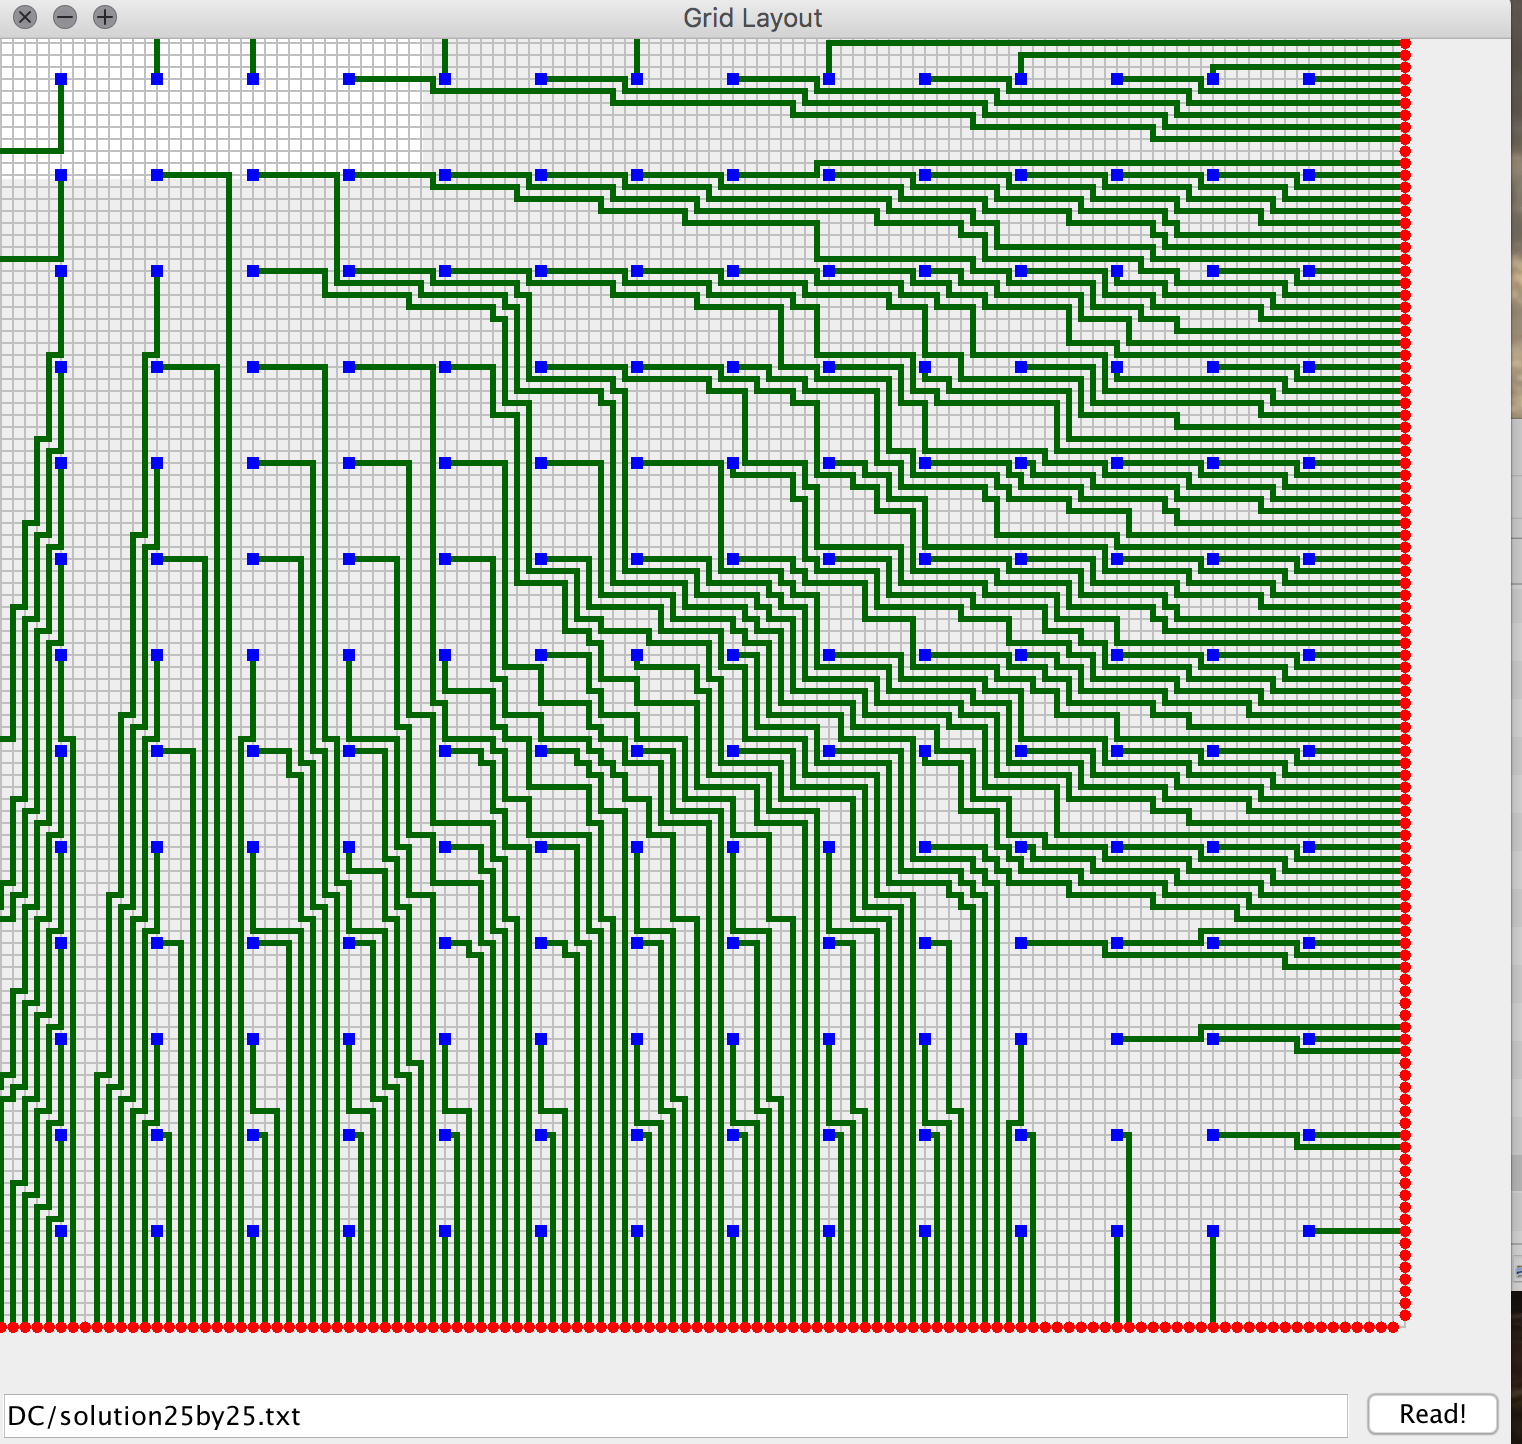
\includegraphics[width = 0.5\textwidth]{ove3.png}
        \caption{Solution at the lower right quarter}
        \label{ZOOM}
    \end{figure}

    We can see a bunch of paths stacking at the diagonal, does it mean that we cannot divide the solution along the diagonal?

    \emph{No}. The key thing to notice is that, the nodes under the diagonal is routed to the bottom, and the nodes above the diagonal is routed to the right.

    For the lower part, we can ``pull'' the paths down to the bottom without changing its length. If a shortest solution exists, there should be one solution, in which the paths are preferrably taking down edges. By doing so we should be able to clear the diagonal, and to judge that no solution exists
    if the paths have to cross over the diagonal.

    Another important observation is that, the nodes at the center axis are spread evenly right and left (this is becuase the axis has $\frac{n}{2}$ nodes, and the gap is about $\frac{n}{4}$), and the nodes at the top of this ``quarter'' mountain are extending their paths to the right, occupying other columns' terminals.
    This is just a heuristics, but turned out to perform quite well.
    \subsubsection{Rules}
    The routing process is done in the following manner. First, we keep a 2D boolean array recording whether a node is visited (similar to BFS).
    \begin{enumerate}[label = \roman*]
        \item Distribute the terminals near at the bottom center to the nodes that are near the center axis.
        \item Search paths one by one for the right half. Prefer down edges to right edges when there are options. Note that sometimes, we need to backtrack, this is not a matter because we never visit a grid twice. \label{ORD}
        \item Then do the same for the left half.
        \item rotate the quarter 3 times to fill the complete board.
    \end{enumerate}
    \begin{figure}[H]
        \centering
        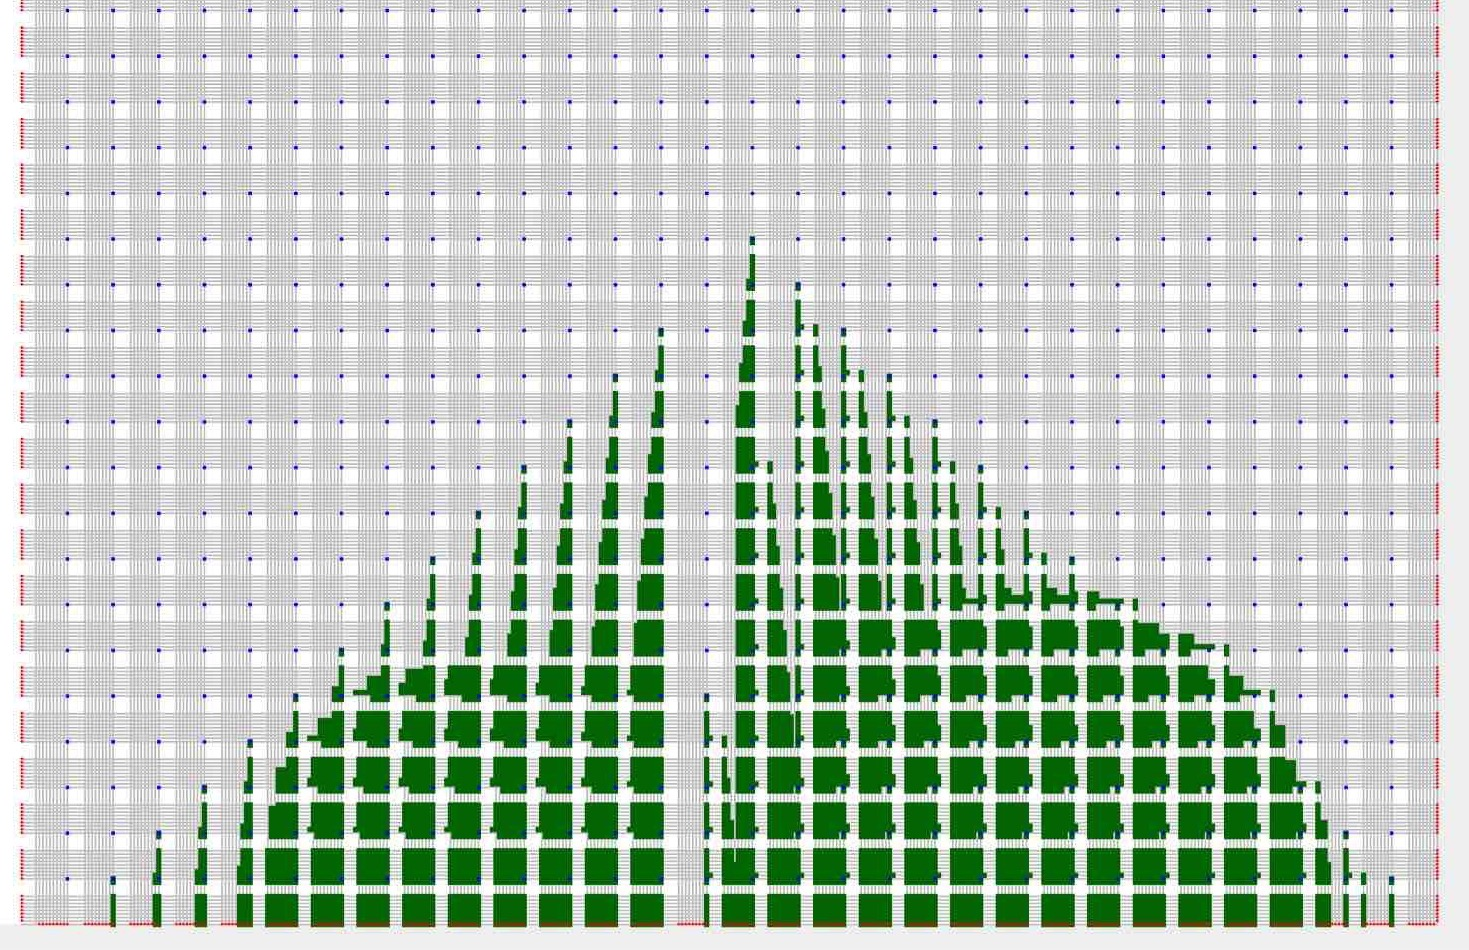
\includegraphics[width = 0.5\textwidth]{QUA1.jpeg}
        \caption{lower quarter (center axis not shown)}
        \label{OB:RULE}
    \end{figure}
    The searching order in \ref{ORD} is not arbitrary. For example, if we route the upper points first, we would have blocked the lower points from escaping. Inspired by Figure \ref{ZOOM}, we devised the following order. (For the right half, same rule for the left half)
    \begin{enumerate}[label = \arabic*]
        \item Route the points column by column, from left to right.
        \item For each column, route the points from bottom to top.
    \end{enumerate}
    As there are not much terminals in each column, we need to ``push'' some paths to the right. Whenever we enter another ``tunnel'' of gap, we need to ensure that the nodes lower in that tunnel are all routed, otherwise we may block these nodes from escaping. This is done
    by making delicate recursive calls and will not be further illustrated in this text, please consult $/src/Rule$ for details.
    \begin{figure}[H]
        \centering
        \begin{subfigure}{0.4\textwidth}
            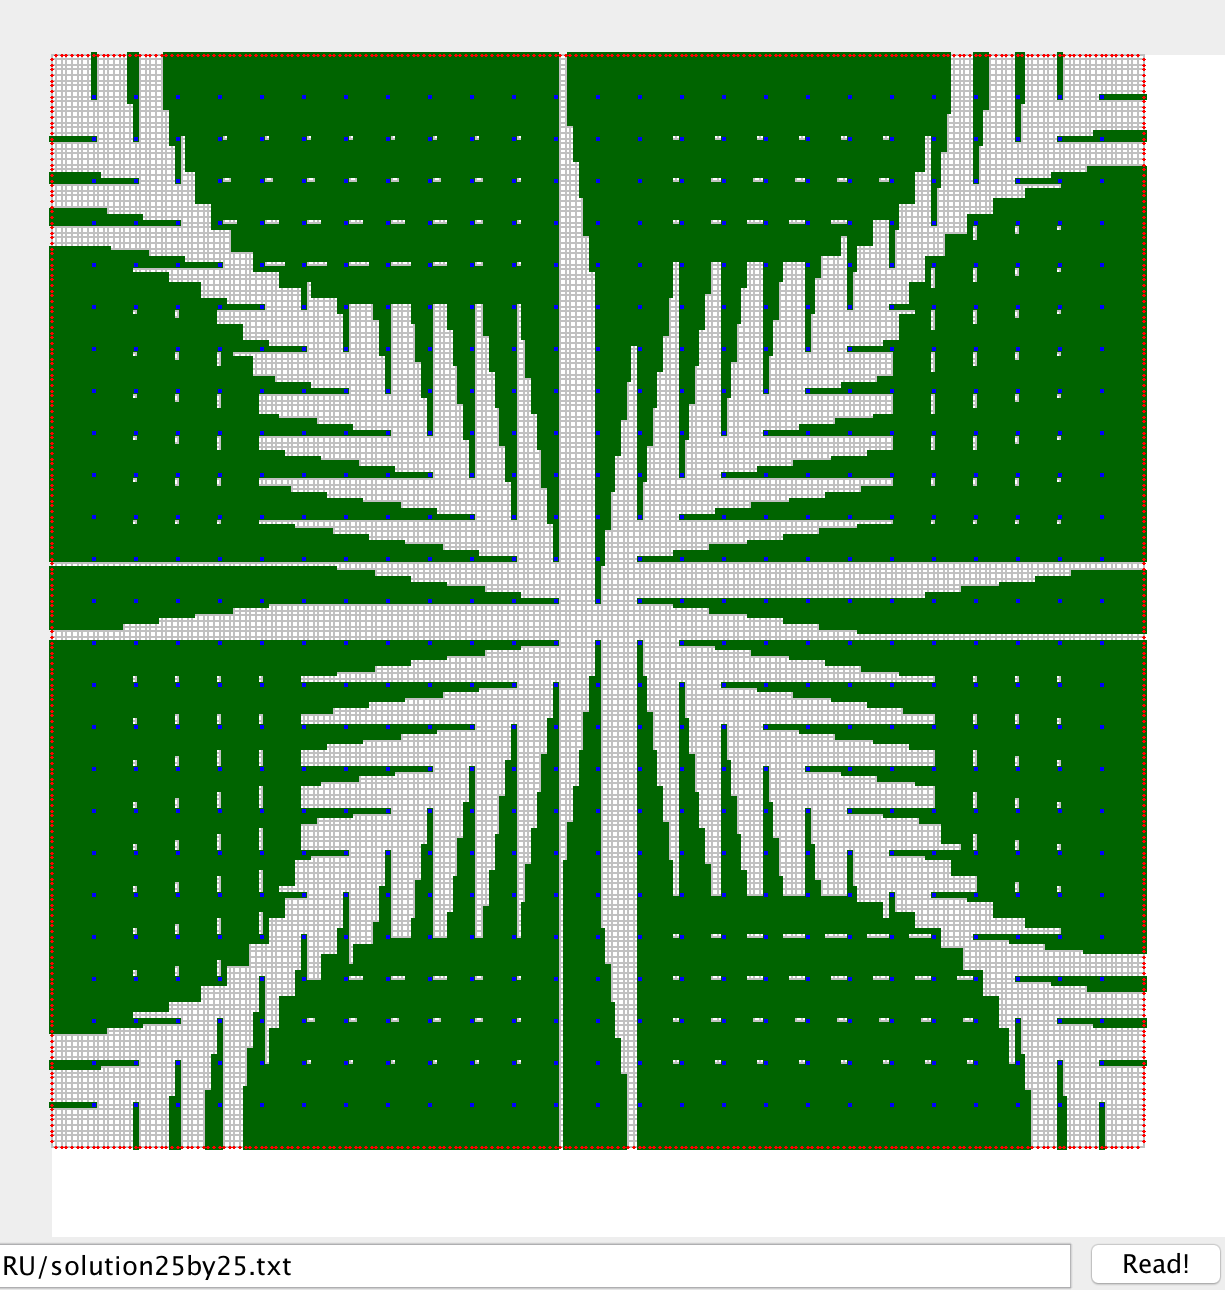
\includegraphics[width = \textwidth]{RU0.png}
            \caption{25 x 25}
        \end{subfigure}
        \begin{subfigure}{0.4\textwidth}
            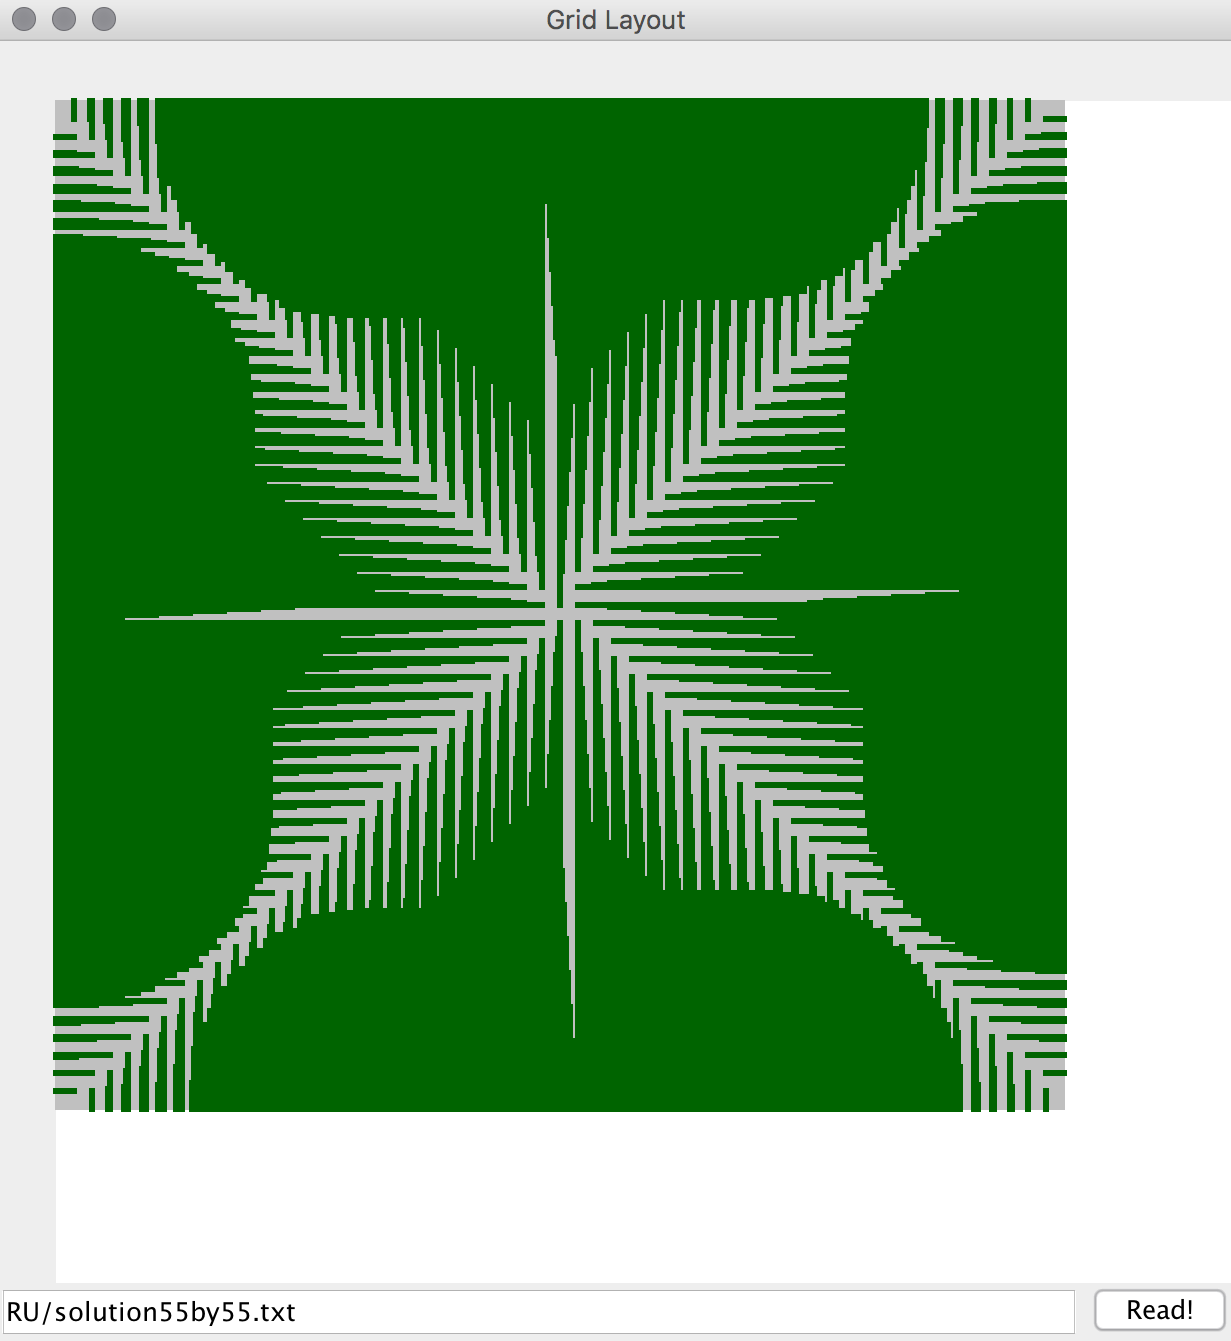
\includegraphics[width = \textwidth]{RU1.png}
            \caption{55 x 55}
        \end{subfigure}
        \begin{subfigure}{0.4\textwidth}
            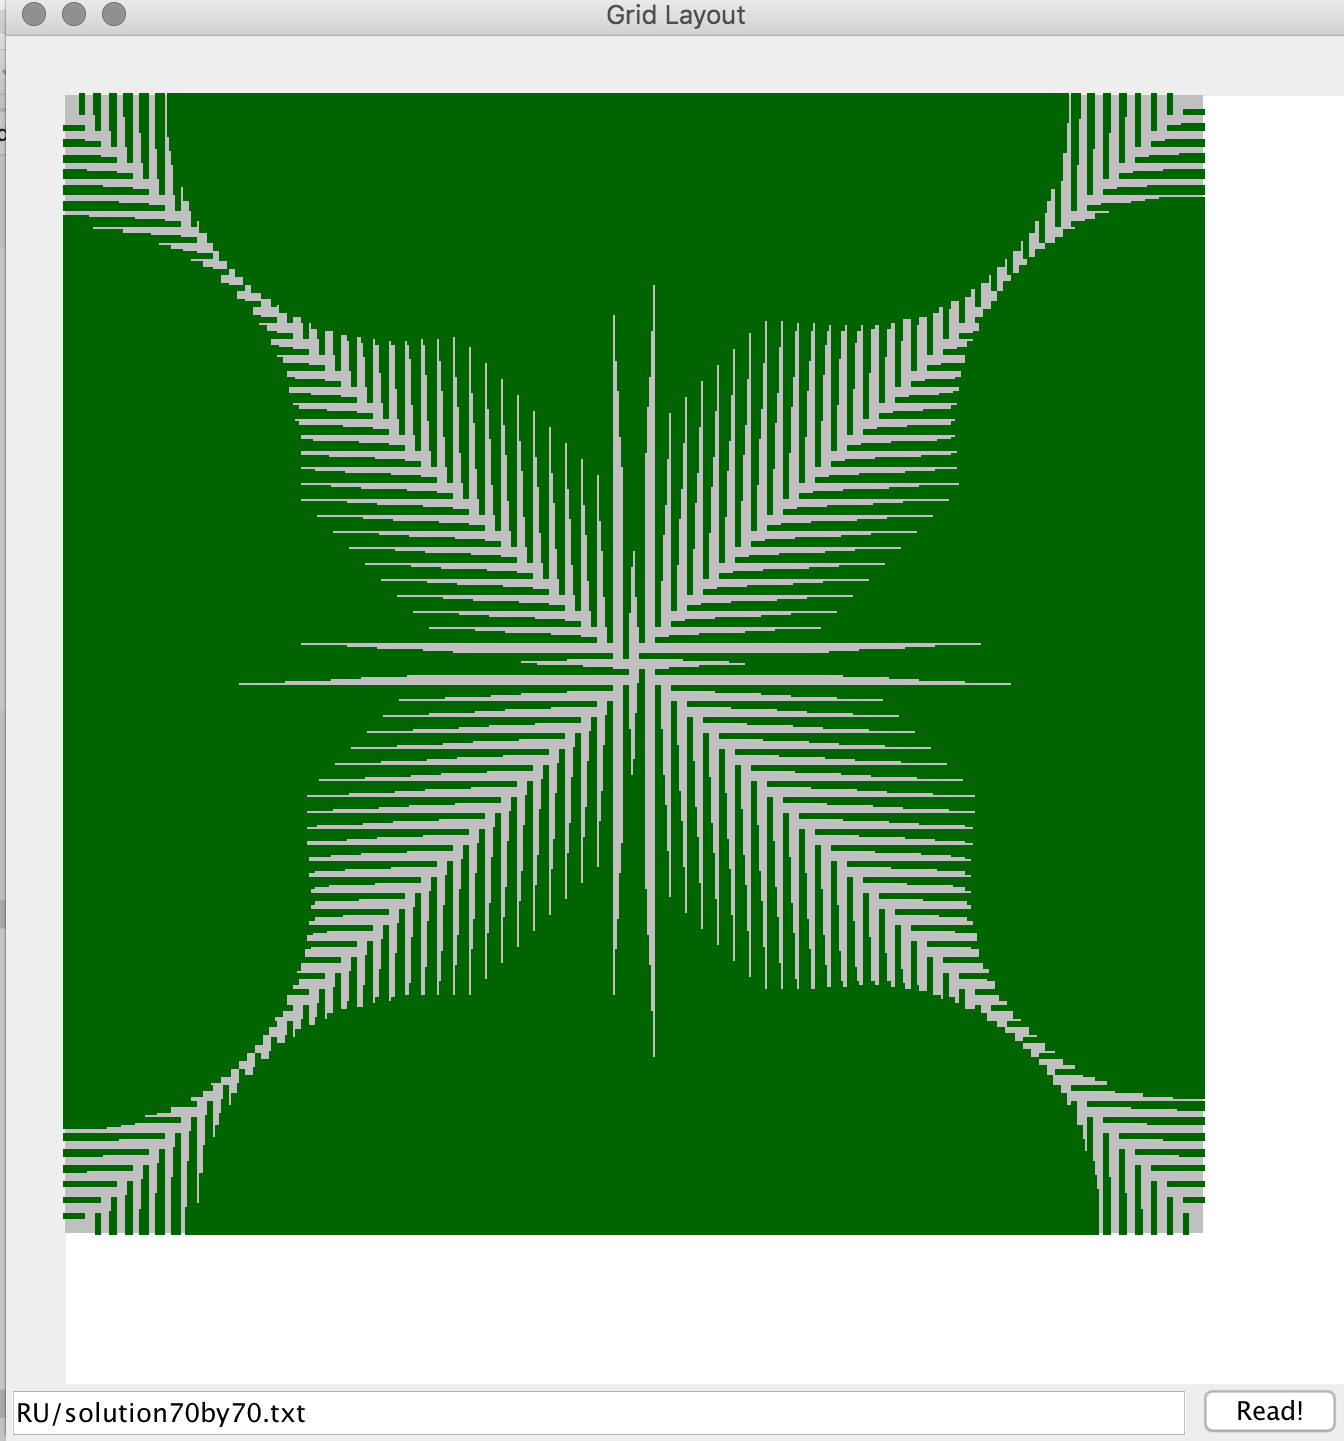
\includegraphics[width = \textwidth]{RU2.png}
            \caption{100 x 100}
        \end{subfigure}
        \begin{subfigure}{0.4\textwidth}
            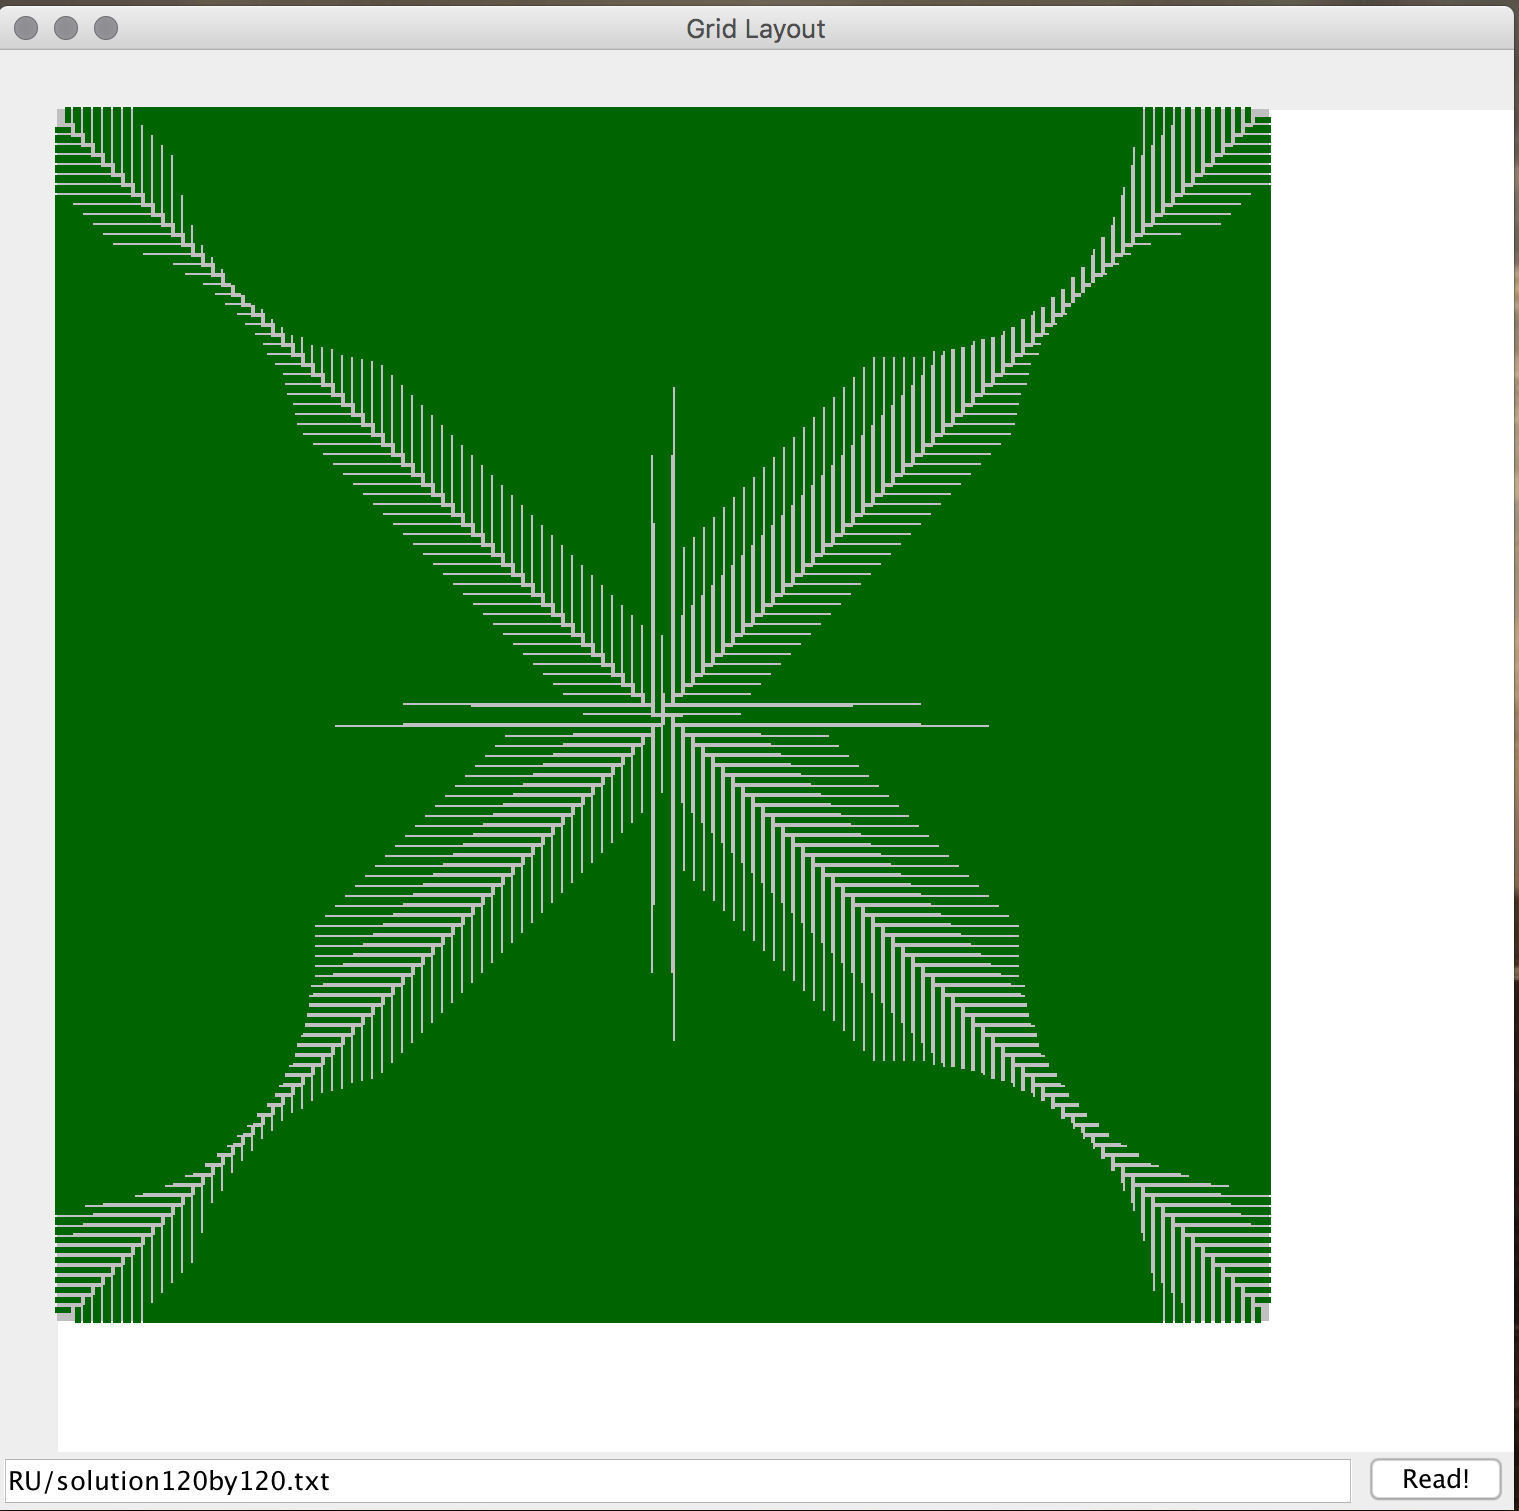
\includegraphics[width = \textwidth]{RU3.png}
            \caption{120 x 120}
        \end{subfigure}
        \caption{RuleRouter with different sizes}
    \end{figure}
    To sum up, the rule router routes the board in a quarter and uses successive path-finding for the terminals. Its main goal is to compress all the paths in a rectangle region (which is nearly visible in Figure \ref{OB:RULE}) so that they do not cross the diagonal. The complexity is $O(l) = O(n^4)$, where $l$ is the total length of the paths. So RuleRouter is significantly faster.
    \section{Result Analysis}
    \subsection{Tables}
    \label{STAT}
    The performance and correctness of different routers are shown in this section.
    \begin{figure}[H]
        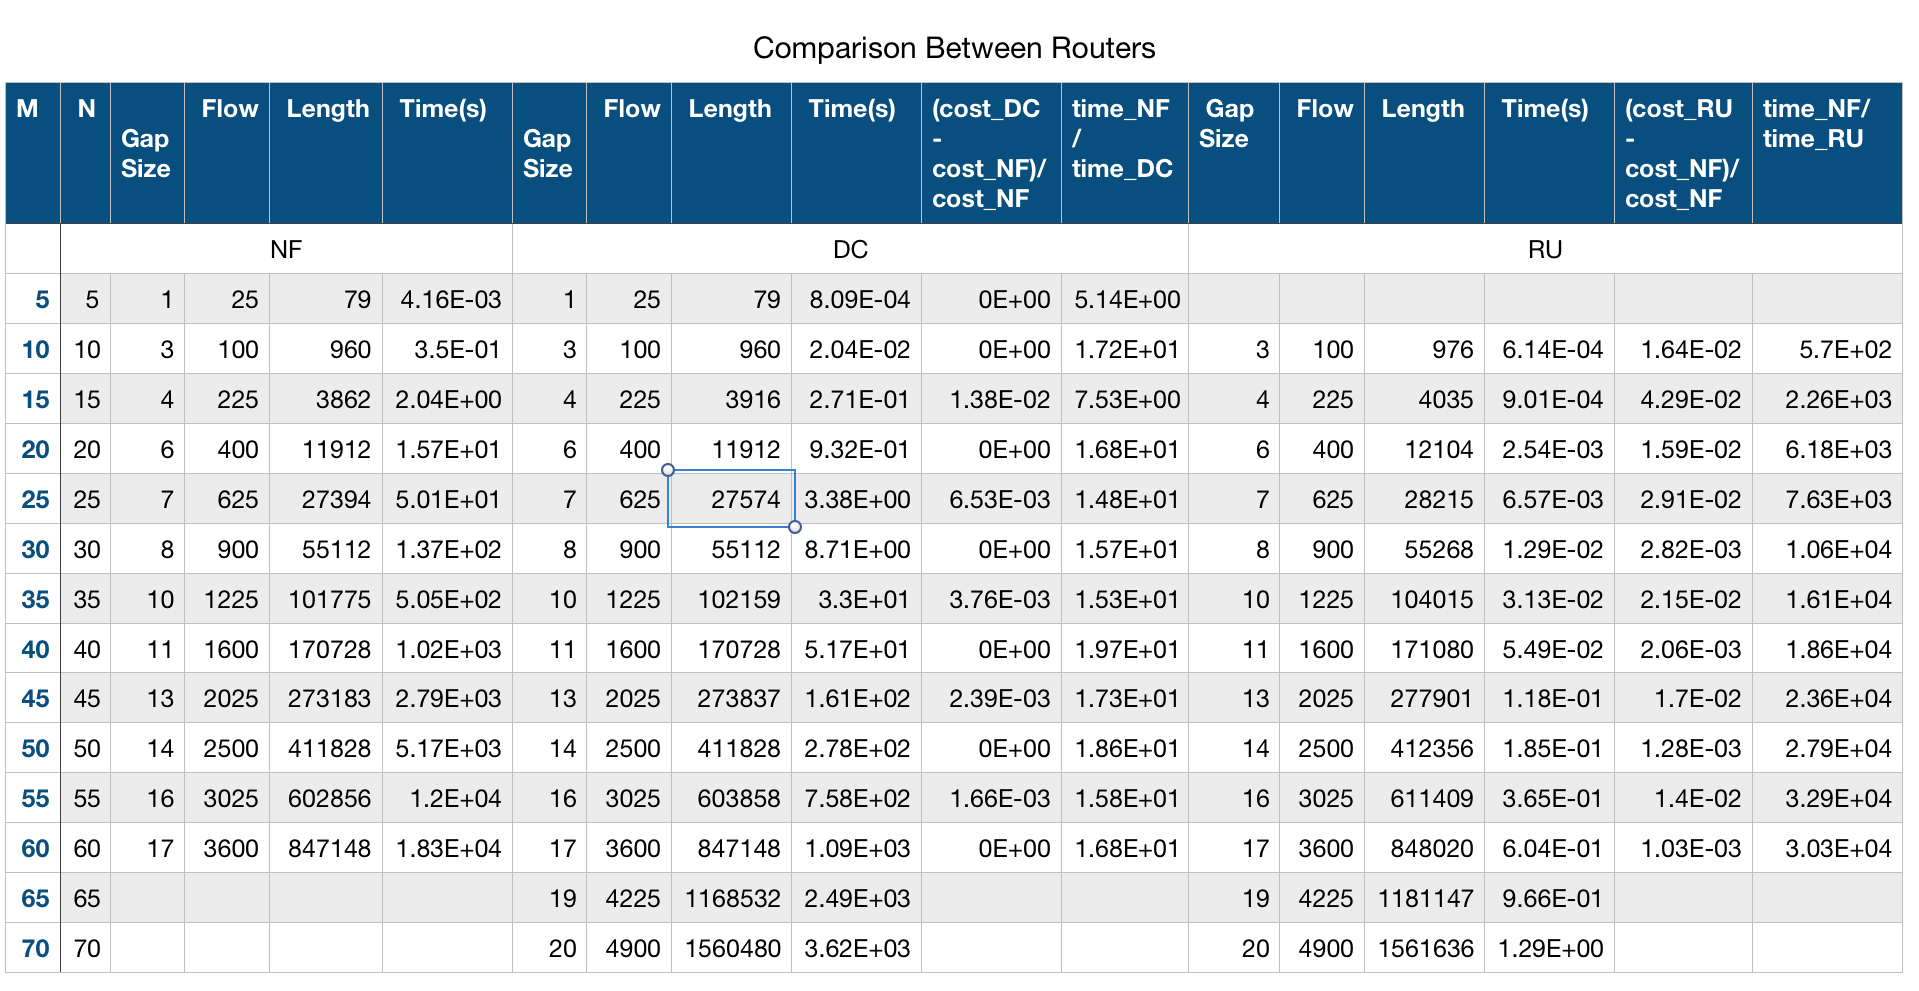
\includegraphics[width = \textwidth]{TABL1.png}
    \end{figure}
    As is shown in the table, the three routers all have the same solution $k$ for the testcases.

    The optimal length is obtained by DCRouter if $n$ is even, and for odd numbers the length is about 0.1 \% longer than optimal, but DCRouter is about 18 times faster.

    For RuleRouter, the length is about 1 \% longer for odd n, and about 0.1 \% longer for even n. However, Rule Router is about 30000 times faster than NFRouter. It uses about 1 second for $65 \times 65 $, which would costs more than 10 hours for NFRouter.
    \begin{table}[H]
        \centering
        \caption{Several other outputs by RuleRouter}
        \csvautobooktabular{RUsamp.csv}
    \end{table}
    \subsection{Validator}
    The validator can be used to verify correctness of results.
    \begin{figure}[H]
        \centering
        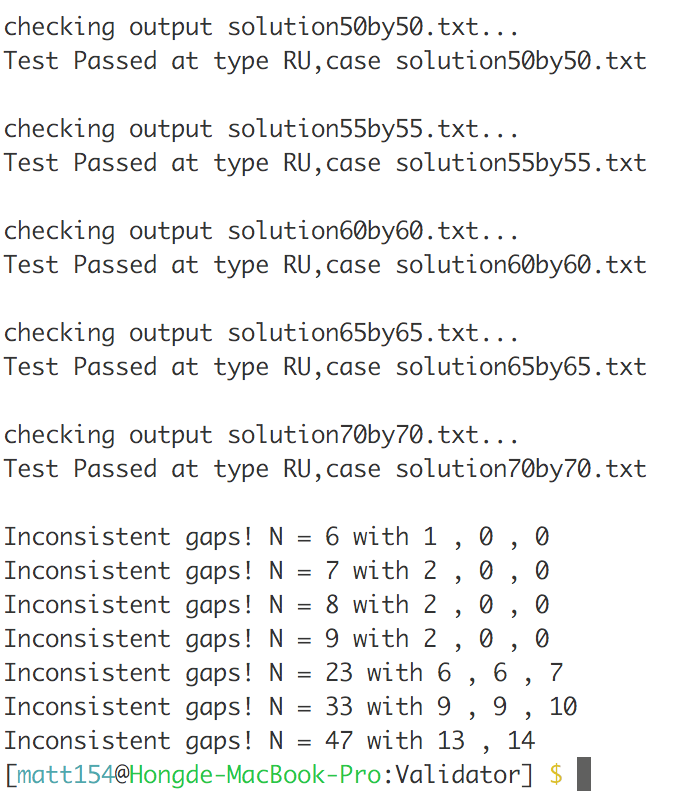
\includegraphics[width = 0.5\textwidth]{VAL.png}
        \caption{Validator (DC, Rule routers not run for $N < 10$)}
    \end{figure}
    As is shown by the validator, all the solutions are valid solutions. However, it turns out that our Rule Router does not always output the minimum $k$ (sometimes off by 1). This phenomenon is rare and occurs only 3 times among all the testcases.
    \section{Conclusion}
    As is illustrated in the text, rule based routing is significantly faster than optimal, network flow based routers. Though suboptimal (about 0.5 \% errors on average), the router can be of great use due to its good efficiency and low error rate.

    \begin{figure}[H]
        \centering
        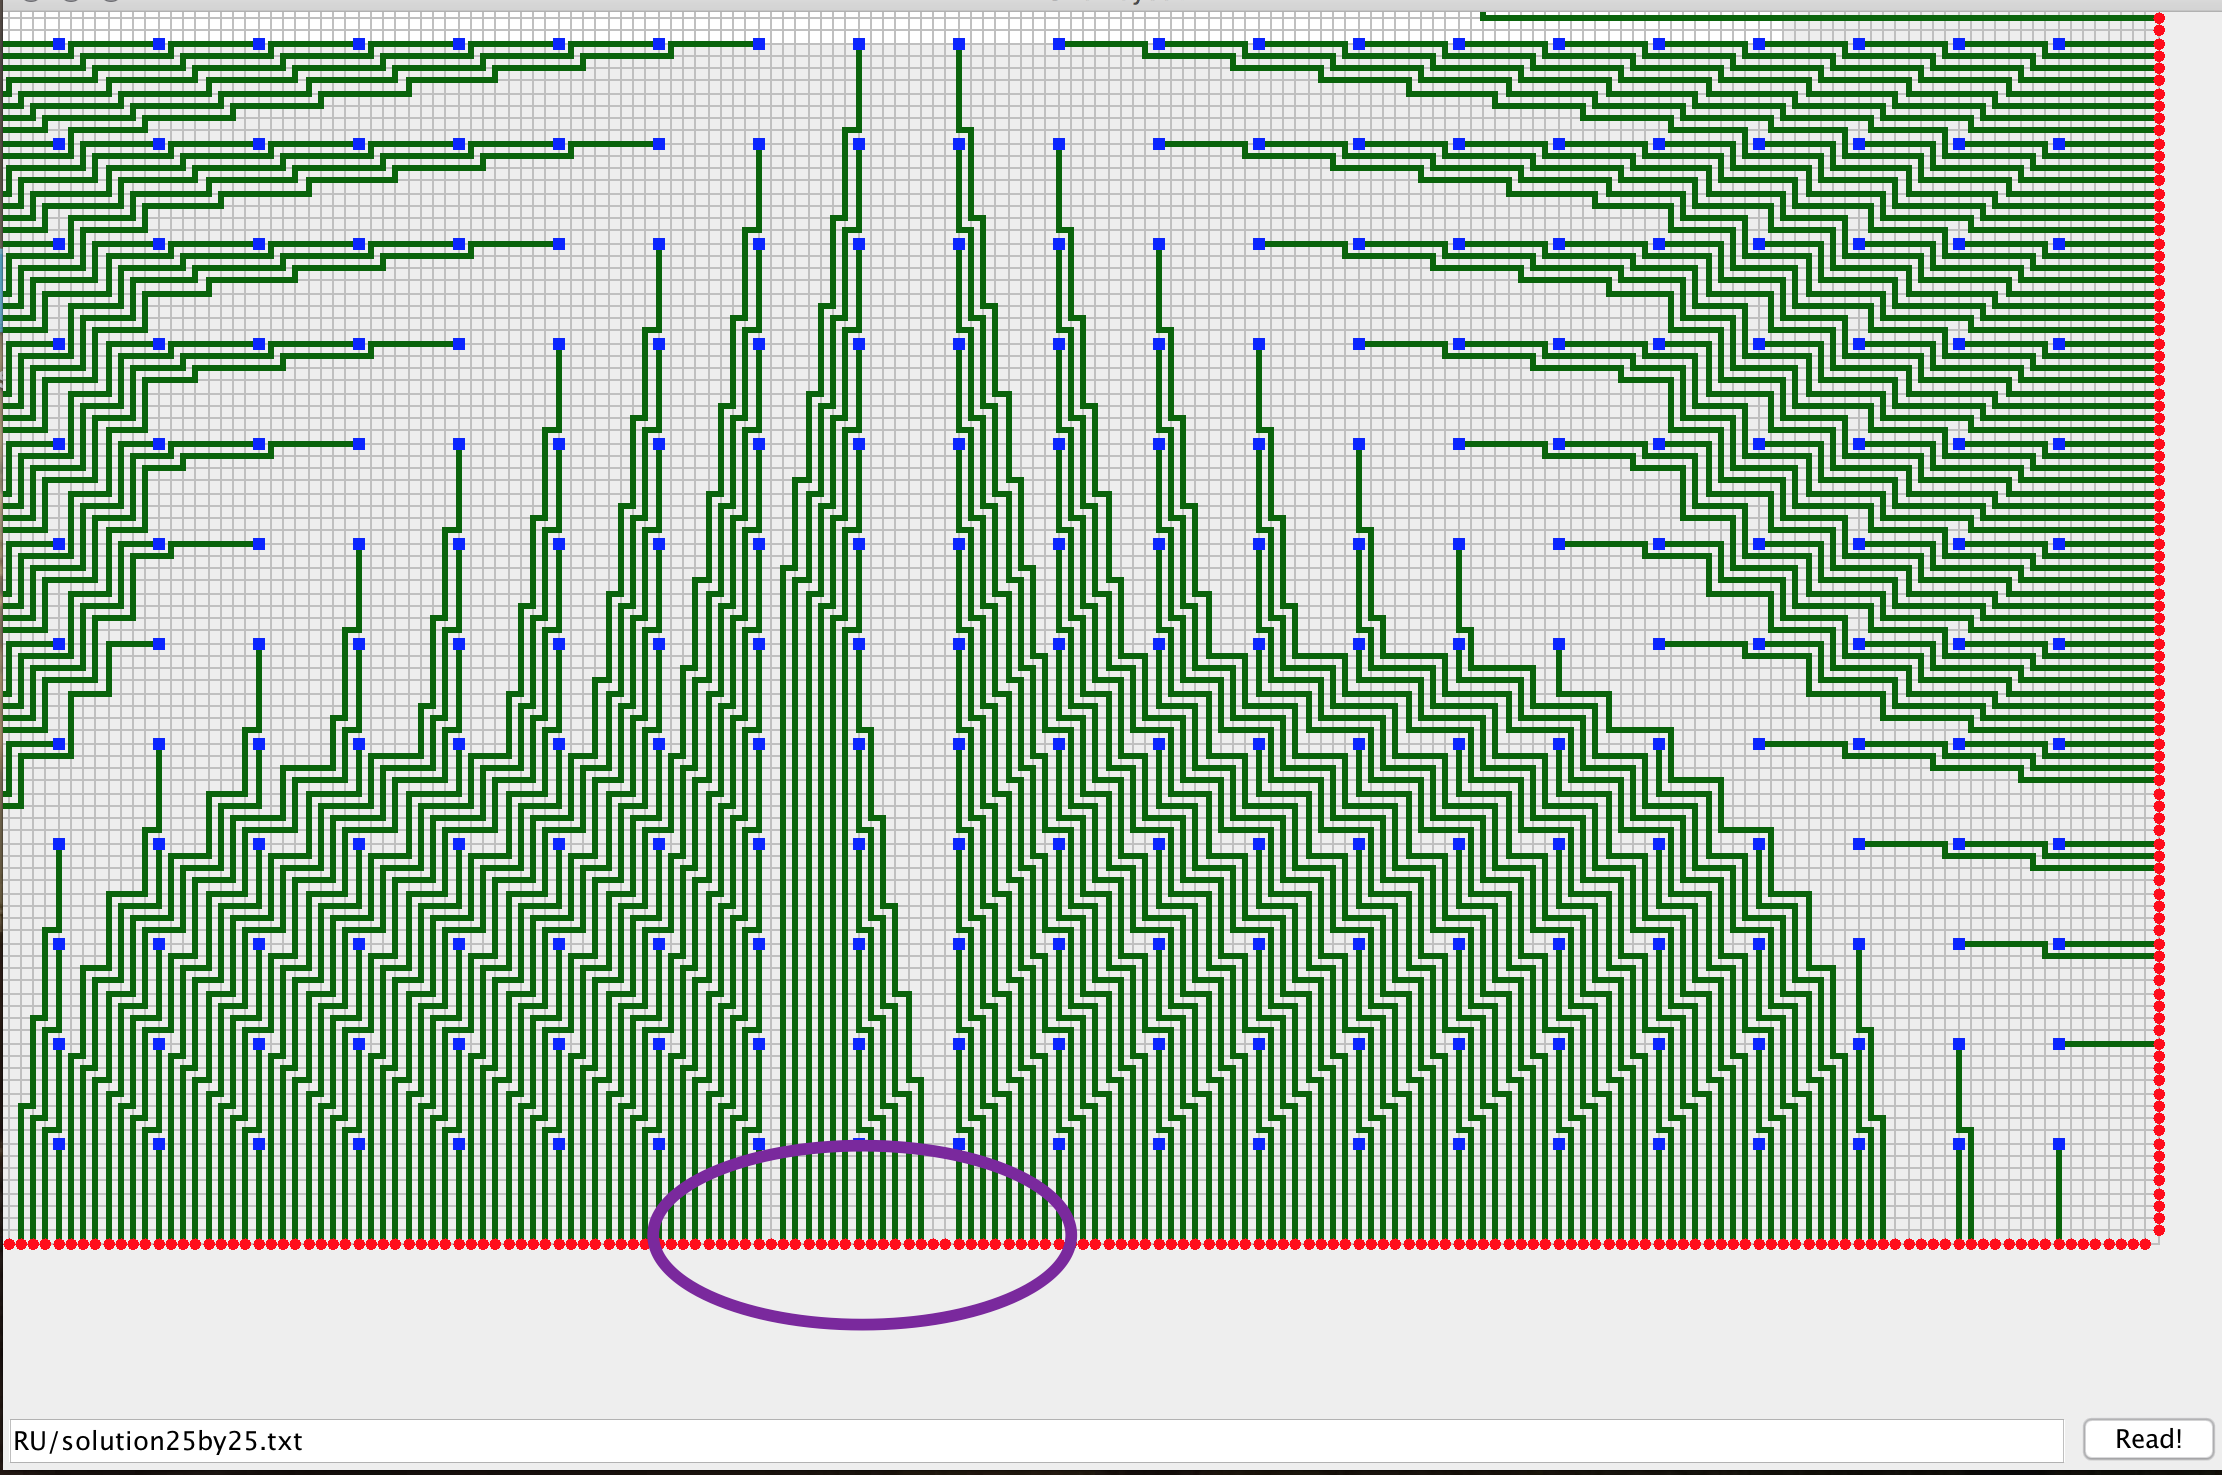
\includegraphics[width = 0.5\textwidth]{CON.png}
        \caption{Unused terminals}
    \end{figure}
    We also want to note that there are still room for improvement. In particular, we should try to fix the center point issue when n is odd (mentioned in Section \ref{DC}, also occured in RuleRouter), which may fix the error in $k$, and bring the 1\% down to 0.1\% for odd n. Also, we notice that there are unused terminals near center axis on the Rule-based solutions.
    If we do more case analysis (which should require \emph{really} delicate, tedious and long codes), we should be able to improve solution's quality.
\end{spacing}
\newpage
\printbibliography
\end{document}

%%%%%%%%%%%%%%%%%%%%%%%%%%%%%%%%%%%%%%%%%%%%%%%%%%%%%%%%%%%%%
